\documentclass[11pt]{article}

\usepackage[margin=1in]{geometry}
\usepackage[T1]{fontenc}
\usepackage{lmodern}
\usepackage{microtype}
\usepackage{amsmath,amssymb,mathtools,bm}
\usepackage{booktabs,longtable,array,tabularx}
\usepackage{enumitem}
\usepackage{graphicx}
\graphicspath{{figures/}{./}}
\usepackage{tikz}
\usepackage{caption}
\usepackage{natbib}
\usepackage[hidelinks]{hyperref}
\usepackage{setspace}
\usepackage{xcolor}

\setstretch{1.08}
\setlength{\parindent}{0pt}
\setlength{\parskip}{0.55em}
\setlist[itemize]{leftmargin=1.5em,itemsep=0.25em,topsep=0.25em}
\setlist[enumerate]{leftmargin=1.7em,itemsep=0.3em,topsep=0.3em}
\renewcommand{\arraystretch}{1.15}

\newcommand{\R}{\mathrm{R}}
\newcommand{\E}{\mathrm{E}}
\newcommand{\I}{\mathbb{I}}
\newcommand{\Exp}{\mathbb{E}}
\newcommand{\Var}{\operatorname{Var}}
\newcommand{\Cov}{\operatorname{Cov}}
\newcommand{\supp}{\operatorname{supp}}
\newcommand{\tr}{\operatorname{tr}}
\newcommand{\diag}{\operatorname{diag}}
\newcommand{\ind}{\mathbb{I}}
\newcommand{\vect}{\operatorname{vec}}
\newcommand{\given}{\,\middle|\,}

\title{\textbf{Covariate-Shift-Adjusted Longitudinal Residual-Rank Screening\\for Selective Borrowing of External Controls}\\[0.5em]
\large A Working Research Blueprint}
\author{}
\date{July 2026}

\begin{document}
\maketitle

\begin{abstract}
This document develops a working methodological plan for selective borrowing of longitudinal external controls. The proposed diagnostic uses residual-trajectory ranks, rather than absolute residual cutoffs, to identify external subjects whose outcomes appear incompatible with randomized controls. The central extension beyond ordinary conformal selective borrowing is adjustment for baseline covariate shift: randomized and external controls are allowed to have different covariate distributions, provided there is overlap and the compatible external outcome law is the same conditional on covariates. A simple split-conformal construction is used for intuition and theory, while the intended implementation uses cross-validated residual scores to avoid wasting a small randomized-control sample. The document distinguishes causal identification assumptions from the weaker object actually screened by a chosen nonconformity score, develops longitudinal score options, studies common-reference versus source-specific covariance standardization, provides an analytically tractable longitudinal data-generating process, and specifies a complete simulation plan with empty result tables.
\end{abstract}

\tableofcontents
\newpage

\section{Provisional project statement}

A concise working description is:

\begin{quote}
We develop a covariate-shift-adjusted longitudinal residual-rank screen for selective borrowing of external controls. Randomized controls provide the reference outcome trajectories. A working longitudinal model produces subject-level nonconformity scores, but the borrowing decision is based on the empirical rank of each external score rather than its raw numerical value. Weighted rank calibration accounts for different baseline covariate distributions across randomized and external sources. After screening, the final source and outcome models are refitted and the retained external controls are incorporated through a longitudinal external-control AIPW estimator.
\end{quote}

The phrase \emph{screening} is preferable to \emph{trimming diagnostic}. In causal-inference writing, ``trimming'' usually evokes removal of units with extreme propensity scores. Here the primary action is outcome-based subject-level screening. The method is conformal in its mathematical calibration, but the substantive description should emphasize what is new relative to existing conformal selective borrowing: covariate-shift adjustment, longitudinal trajectory scores, and integration with a refitted longitudinal borrowing estimator.

A suitable provisional title is:

\begin{quote}
\textbf{Covariate-shift-adjusted longitudinal residual-rank screening for selective borrowing of external controls.}
\end{quote}

This is a working positioning, not yet a finalized novelty claim. Ordinary residual-rank selective borrowing has already been developed by \citet{zhu2025csb}; weighted conformal calibration under covariate shift has also been developed in the conformal literature \citep{tibshirani2019weighted,jin2026weighted}. The likely contribution is their longitudinal, estimand-aware integration in the external-control setting, together with a careful study of which compatibility notion the screen does and does not diagnose.

\section{Scientific motivation}

\subsection{Why longitudinal outcomes matter}

Let the post-baseline untreated or treated outcome trajectory be
\[
\bm Y(a)=\{Y_1(a),\ldots,Y_T(a)\}^{\top}, \qquad a\in\{0,1\}.
\]
The trial-population longitudinal treatment-effect vector is
\[
\bm\tau=\Exp_{\R}\{\bm Y(1)-\bm Y(0)\}.
\]
A prespecified clinical contrast is
\[
\tau_c=c^{\top}\bm\tau
=\Exp_{\R}\!\left[c^{\top}\{\bm Y(1)-\bm Y(0)\}\right].
\]
Examples include:
\begin{itemize}
    \item final visit: $c=(0,\ldots,0,1)^{\top}$;
    \item final-minus-baseline change: $c=(-1,0,\ldots,0,1)^{\top}$ when baseline is included in $\bm Y$;
    \item average response over follow-up: $c=(1/T,\ldots,1/T)^{\top}$;
    \item an area-under-the-curve contrast using numerical-integration weights;
    \item a prespecified linear slope contrast.
\end{itemize}

Longitudinal data are valuable for more than simply creating several endpoints.

First, they describe the temporal pattern of response. Two control sources can agree at the final visit but differ in early decline, recovery, slope, curvature, or persistence. Such discrepancies may matter scientifically and may also reveal incompatibility that a scalar endpoint cannot see.

\begin{figure}[ht]\centering

\includegraphics[width=\linewidth]{fig_long.pdf}
\caption{Why the screen must be longitudinal, and why the nonconformity score must match the drift. The shaded band is the range of randomized controls (the natural progression); \emph{most} external controls are compatible (blue) and track it, while a \emph{few} are incompatible (amber) and drift away in different shapes. \emph{Left:} late deterioration---identical early, diverging only at later visits, so a single early visit misses it while the visit-average and slope contrasts catch it. \emph{Middle:} a global level shift---seen by the baseline and visit-average contrasts but not the slope. \emph{Right:} a transient dip that recovers---invisible to the baseline, the endpoint, and (on net) the visit-average, caught only by a trajectory-shape (Mahalanobis) score. No single scalar endpoint reveals all three: the score must be aligned to the estimand and the anticipated drift shape.}
\label{fig:long}
\end{figure}

Second, repeated measurements provide within-subject information. If the covariance structure is modeled adequately, correlated measurements can improve precision relative to discarding all but one visit.

Third, longitudinal data make the external-control problem harder. The analyst must address time-dependent variability, within-subject covariance, irregular visit timing, intermittent missingness, dropout, and possibly source-specific measurement processes. Real-world data can be especially heterogeneous in these respects.

The longitudinal focus is also aligned with the existing FDA-supported external-control project. The JRSS-A work of \citet{zhou2025causal} studies randomized trials with longitudinal outcomes and was partially supported by FDA/HHS cooperative agreement U01 FD007206. This motivates the longitudinal direction, but the scientific rationale above should remain the main argument rather than a broad claim about FDA priorities.

\subsection{Why selective borrowing is needed for real-world external controls}

External controls may arise from previous trials, registries, electronic health records, or natural-history studies. Compared with a closely harmonized historical randomized trial, real-world controls may differ in:
\begin{itemize}
    \item baseline disease severity and prognostic factors;
    \item visit schedules and observation frequency;
    \item endpoint collection, measurement error, and adjudication;
    \item missingness and dropout mechanisms;
    \item calendar time, standard of care, and concomitant treatment;
    \item conditional outcome means, variances, correlations, or tails.
\end{itemize}

Full borrowing can improve precision when external controls are compatible, but can introduce bias when incompatibility remains after adjustment. The scientific question is therefore not merely whether to use external data, but which external subjects carry credible information for the randomized trial population.

\begin{figure}[ht]\centering

\includegraphics[width=\linewidth]{fig_design.pdf}
\caption{The borrowing problem at a glance. A randomized trial supplies a valid but small control arm; a large external source (registry, historical arm, EHR) could enlarge it, but the two sources differ in baseline case-mix (covariate shift) and a hidden subset of external controls is incompatible (a shifted control-outcome law). The proposed method screens each external control by ranking it against the randomized controls, borrows the compatible ones into the control comparison, and drops the rest, so borrowing sharpens $\widehat\tau$ without importing bias.}
\label{fig:design}
\end{figure}

\section{Identification assumptions and diagnostic targets}

\subsection{Notation}

Let $S=1$ denote the randomized trial and $S=0$ the external source. Within the trial, $A=1$ denotes randomized treatment and $A=0$ randomized control. Screening uses the randomized controls and external controls, both observed under control.

Let $X$ denote baseline covariates measured comparably in both sources. The main causal target is $\tau_c$ in the randomized-trial population.

\subsection{Four distinct compatibility concepts}

These concepts should not be conflated.

\paragraph{1. Covariate overlap.}
For external controls to inform the trial population, the relevant trial covariate support must be represented externally:
\[
\supp\{X\mid S=1\}\subseteq \supp\{X\mid S=0\},
\]
or at minimum the analysis must be restricted to a common-support region. Importantly, overlap does \emph{not} require the two covariate distributions to be equal:
\[
f_{\R}(x)\neq f_{\E}(x)
\]
is allowed. This distinction is central to the proposed weighted calibration.

\paragraph{2. Conditional mean compatibility for one contrast.}
For identification of the untreated mean of a specific contrast $c^{\top}\bm Y(0)$, a sufficient assumption is
\[
\Exp\{c^{\top}\bm Y(0)\mid X,S=1\}
=
\Exp\{c^{\top}\bm Y(0)\mid X,S=0\}.
\tag{ME-$c$}
\]
This condition can hold even if conditional variances, correlations, tails, or other trajectory features differ.

\paragraph{3. Vector conditional mean compatibility.}
If all linear trajectory contrasts are of interest, a stronger mean condition is
\[
\Exp\{\bm Y(0)\mid X,S=1\}
=
\Exp\{\bm Y(0)\mid X,S=0\}.
\tag{VME}
\]

\paragraph{4. Conditional distribution compatibility.}
The stronger distribution-level condition is
\[
\bm Y(0)\mid X,S=1
\ \overset{d}{=}\ 
\bm Y(0)\mid X,S=0.
\tag{DE}
\]
The JRSS-A paper uses a conditional distributional ignorability condition of this form through $\bm Y(0)\perp S\mid X$ \citep{zhou2025causal}. The CSB paper explicitly distinguishes full exchangeability, needed for ordinary conformal rank validity, from the weaker mean exchangeability used to identify an average treatment effect \citep{zhu2025csb}.

The logical relation is
\[
\text{DE}\quad\Longrightarrow\quad\text{VME}\quad\Longrightarrow\quad\text{ME-$c$},
\]
but neither reverse implication holds in general.

\begin{figure}[ht]\centering
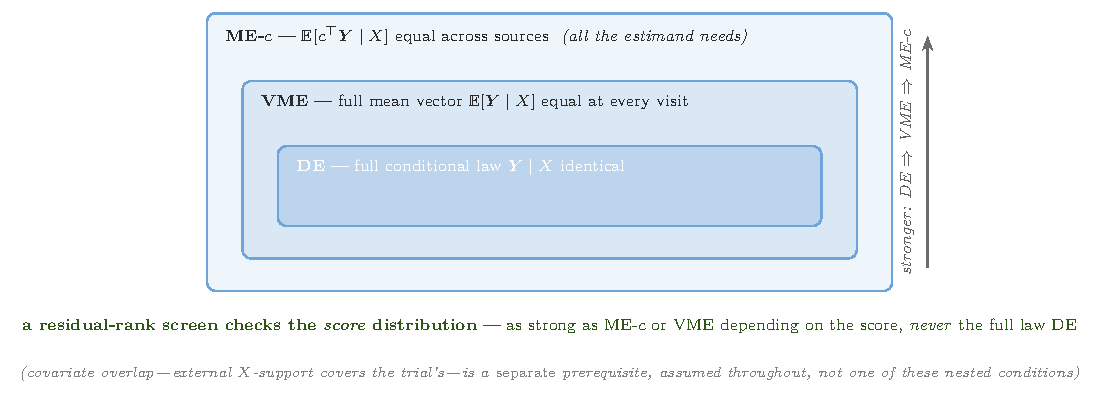
\includegraphics[width=0.96\linewidth]{fig_compat.pdf}
\caption{The four compatibility concepts are nested, from the weakest (covariate overlap, outermost) to the strongest (full conditional-law equality, innermost): $\text{DE}\Rightarrow\text{VME}\Rightarrow\text{ME-}c$, all presuming overlap. Identifying the treatment effect needs only level~2 (ME-$c$); ordinary conformal rank validity nominally needs level~4. A residual-rank screen on a chosen nonconformity score checks the \emph{score} distribution---an object as strong as level~2 or~3 depending on the score---so it can control borrowing bias without asserting the full-law equality of level~4.}
\label{fig:compat}
\end{figure}

\subsection{What a residual-rank screen actually diagnoses}

Let a fitted working model and scale/covariance model define a scalar nonconformity score
\[
V=s\{\bm Y,X;\widehat\eta\}.
\]
A screen based on $V$ does not directly verify DE. Its immediate null is score compatibility:
\[
V\mid X,S=1\ \overset{d}{=}\ V\mid X,S=0.
\tag{SE}
\]
If DE holds and the same fixed scoring rule is applied in both sources, then SE holds. Thus DE is sufficient for score compatibility. The converse is false: different longitudinal distributions can map to the same one-dimensional score distribution.

Accordingly, the method should be described as follows:

\begin{quote}
The screen evaluates residual-trajectory compatibility with randomized controls under a chosen score. Passing the screen does not establish conditional distributional exchangeability. The procedure can reduce bias when external incompatibility manifests through the selected nonconformity score.
\end{quote}

A failed screen also requires careful interpretation. A whole-trajectory Mahalanobis score may detect a variance or covariance difference that does not bias the mean contrast $\tau_c$. This is why score choice is a substantive design decision, not only a technical one.

\section{Existing design-stage screen: propensity-score trimming}

Define the source propensity score
\[
e(X)=\Pr(S=1\mid X).
\]
Propensity-score matching, weighting, and trimming are classical tools for balancing measured baseline covariates \citep{rosenbaum1983,crump2009}. Extreme $e(X)$ values identify regions in which one source has little density relative to the other because
\[
\frac{f_{\R}(x)}{f_{\E}(x)}
=
\frac{1-\Pr(S=1)}{\Pr(S=1)}
\frac{e(x)}{1-e(x)}.
\]

Propensity-score trimming therefore targets covariate overlap or practical positivity. It does not directly assess whether
\[
\bm Y(0)\mid X,S=1
\]
and
\[
\bm Y(0)\mid X,S=0
\]
are compatible. This provides a natural bridge to outcome-based residual-rank screening:
\[
\begin{array}{ccl}
\text{propensity-score trimming} &:& X\text{-overlap},\\[0.2em]
\text{residual-rank screening} &:& \bm Y\mid X\text{-compatibility through }V.
\end{array}
\]

The two steps are complementary. Units outside the trial's covariate support should not be rescued by an outcome screen, while units with adequate $X$ support may still show incompatible control trajectories.

\section{Basic idea for a broad audience: scalar outcome and no covariates}

This section deliberately uses the simplest setting. Its purpose is explanation and visualization, not the final method.

Suppose an outcome model is fitted using randomized controls. For each randomized control in a calibration sample, calculate an absolute residual
\[
V_i^{\R}=|Y_i^{\R}-\widehat m|.
\]
For external subject $j$, calculate
\[
V_j^{\E}=|Y_j^{\E}-\widehat m|.
\]
The external subject is not judged by whether $V_j^{\E}$ exceeds a fixed number such as 2 or 3. Instead, it is judged by where its residual ranks among randomized-control residuals:
\[
p_j=
\frac{1+\sum_{i=1}^{n_C}\ind(V_i^{\R}\ge V_j^{\E})}{n_C+1}.
\tag{1}
\]
A small $p_j$ means that almost no randomized control has a residual as large as the external subject's residual.

\begin{figure}[ht]
\centering
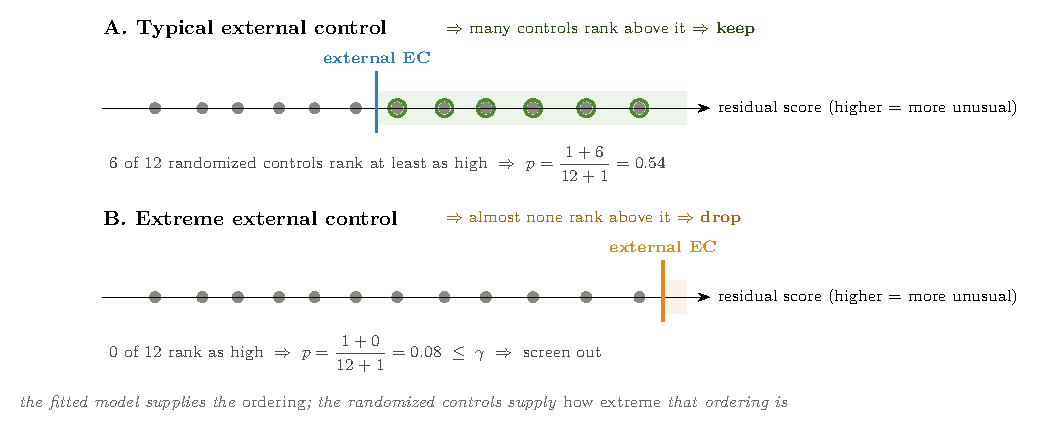
\includegraphics[width=0.92\linewidth]{fig_rank.pdf}
\caption{Residual ranking, not an absolute residual cutoff. Each external control's score is placed among the randomized-control calibration scores; its conformal $p$-value is $(1+\#\{\text{controls at least as extreme}\})/(n_C+1)$. A typical external control~(A) has many controls ranking above it ($p$ large $\Rightarrow$ retain); an extreme one~(B) has almost none ($p\le\gamma\Rightarrow$ screen out). The fitted model supplies the \emph{ordering}; the randomized controls supply \emph{how extreme} that ordering is.}
\label{fig:basicrank}
\end{figure}

Conditionally on the fitted model, if the external subject and calibration controls are exchangeable, their scores are exchangeable even when the fitted model is misspecified. With no ties, the rank of the external score among $n_C+1$ scores is discrete uniform. Thus the split-conformal $p$-value is super-uniform, as formalized for CSB by \citet{zhu2025csb}.

This simple figure communicates the key idea to a wider audience: the outcome model supplies a useful ordering, while rank calibration determines whether the external observation is unusually incompatible relative to actual randomized controls.

\section{Why rank calibration is preferable to direct prediction residuals}

This is a core motivation and should be emphasized, not relegated to a minor caveat.

\subsection{Direct standardized-residual screening}

A seemingly simpler approach is:
\begin{enumerate}
    \item fit a longitudinal model on randomized controls;
    \item predict each external trajectory;
    \item compute a raw or standardized residual;
    \item delete an external subject whenever the residual exceeds a fixed threshold.
\end{enumerate}

For example, one might declare
\[
\max_t\left|
\frac{Y_{jt}^{\E}-\widehat m_t(X_j)}{\widehat\sigma_t(X_j)}
\right|>2
\]
to be incompatible. Such a rule requires the fitted mean and scale models to be accurate enough that the numerical threshold has a valid interpretation. If the mean model omits nonlinear time trends or interactions, or if the scale model understates variability, compatible external subjects can appear artificially extreme.

\subsection{The conformal rank principle}

Let the true conditional outcome law be arbitrary. After cross-fitting or sample splitting, regard the working model $\widehat\eta$ as fixed and define
\[
V=s\{\bm Y,X;\widehat\eta\}.
\]
Under conditional compatibility,
\[
\bm Y^{\R}\mid X=x
\overset d=
\bm Y^{\E}\mid X=x.
\]
Therefore, for any fixed scoring rule, correct or incorrect,
\[
\Pr(V^{\R}\le v\mid X=x)
=
\Pr(V^{\E}\le v\mid X=x).
\tag{2}
\]
The fitted model need not equal the true outcome model for this equality. Misspecification affects both compatible randomized and external subjects through the same score map.

The advantage of rank calibration is therefore precise:
\begin{itemize}
    \item no normality or chi-square reference distribution is required for the raw score;
    \item no universal numerical cutoff is required;
    \item systematic working-model error shared by compatible randomized and external controls is empirically represented in the randomized-control score distribution;
    \item model quality primarily affects the ability to separate incompatible from compatible controls, that is, power, rather than oracle null calibration.
\end{itemize}

\begin{figure}[ht]\centering
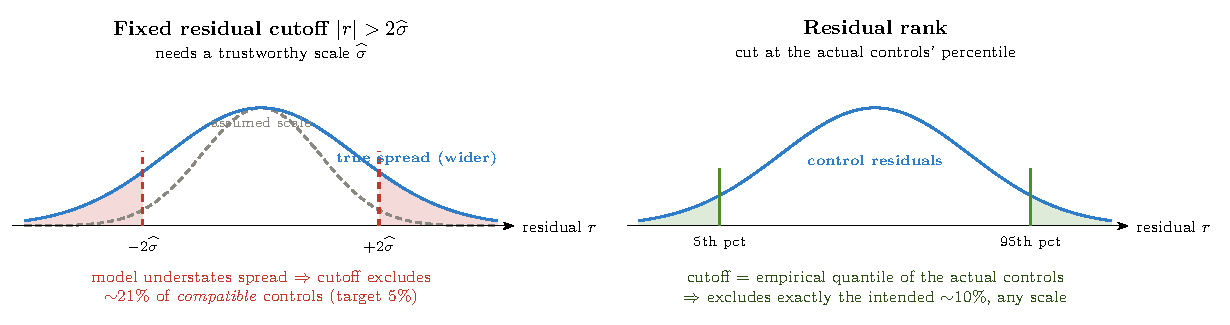
\includegraphics[width=\linewidth]{fig_rankres.pdf}
\caption{Why rank, not a raw residual cutoff. \emph{Left:} a fixed rule $|r|>2\widehat\sigma$ trusts the model's scale $\widehat\sigma$; if the working model understates the true spread, the cutoff sits too close to the center and excludes a large fraction of \emph{compatible} controls (here $\sim$$21\%$ against a $5\%$ target). \emph{Right:} ranking each residual among the actual randomized-control residuals puts the cutoff at an empirical quantile of those controls, so the excluded fraction is the intended one \emph{whatever} the true scale---the calibration is done by the data, not by a trusted number.}
\label{fig:rankres}
\end{figure}

\begin{figure}[ht]\centering
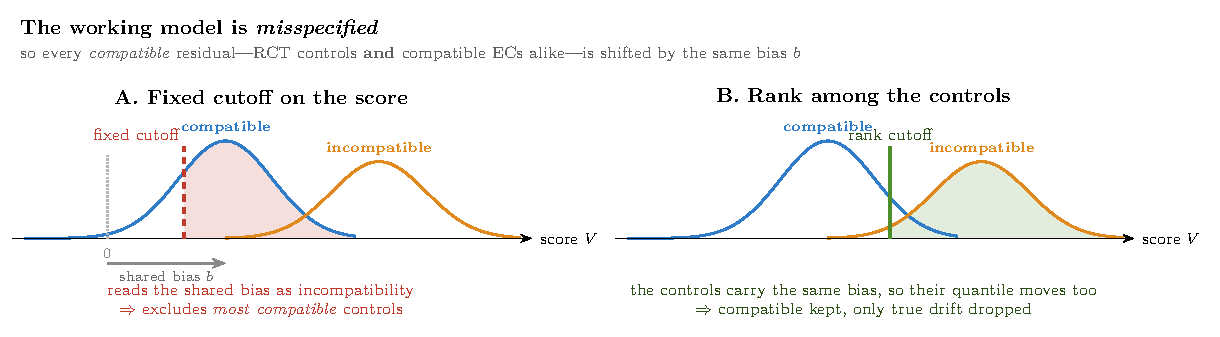
\includegraphics[width=\linewidth]{fig_misspec.pdf}
\caption{Rank calibration is robust to model \emph{misspecification}---the deeper reason to rank rather than threshold the residual value itself. A wrong working mean model shifts \emph{every} compatible residual---randomized controls and compatible external controls alike---by the same bias $b$, because both share the true conditional law and pass through the same (misspecified) score map. \emph{A:} a fixed cutoff, calibrated as if the model were correct, reads that shared bias as incompatibility and excludes most compatible controls. \emph{B:} because the randomized controls carry the same bias, their empirical quantile moves with them, so ranking against them cancels the shared error and flags only genuinely different external controls. This is the conformal exchangeability guarantee (eq.~(2)): the $p$-value stays valid under \emph{any} working model, correct or not---the scale robustness of Figure~\ref{fig:rankres} is a special case.}
\label{fig:misspec}
\end{figure}

This does not make the outcome model irrelevant. A very poor model produces broad, noisy randomized-control scores, so genuine external drift may no longer rank as extreme. A poor scale model may also emphasize the wrong visits or covariate regions. Cross-fitting is important because in-sample residuals from a flexible model can be too optimistic.

The central distinction is:
\[
\begin{array}{ccl}
\text{direct residual threshold} &:& \text{requires a trustworthy numerical scale},\\
\text{residual rank} &:& \text{calibrates that scale empirically against randomized controls}.
\end{array}
\]

\section{Proposed full method}

The full method has six moves, summarized in Figure~\ref{fig:pipeline}: using the randomized controls, fit a working control-mean model, residualize, and reduce each trajectory to an estimand-aligned nonconformity score; then rank each external control against the randomized controls with covariate-shift weighting, screen conservatively, and refit a transported borrowing estimator on the survivors. The subsections below develop each step in turn.

\begin{figure}[ht]\centering

\includegraphics[width=\linewidth]{fig_pipeline.pdf}
\caption{The proposed method in six steps. Steps 1--3 (\emph{learn}) fit a control-mean model on the randomized controls, residualize every control trajectory, and reduce it to an estimand-aligned score. Steps 4--5 (\emph{flag}) rank each external control's score against the randomized-control scores---reweighted by the covariate-shift density ratio $\omega_0$---and keep only those with a large conformal $p$-value under a symmetric, adaptive threshold. Step 6 (\emph{borrow}) refits a transported AIPW on the randomized controls plus the retained external controls, yielding $\widehat\tau$ and a confidence interval.}
\label{fig:pipeline}
\end{figure}

\subsection{Step 1: prespecify the estimand and harmonize the data}

Choose a primary contrast $c$ and target
\[
\tau_c=\Exp_{\R}\!\left[c^{\top}\{\bm Y(1)-\bm Y(0)\}\right].
\]
Before outcome screening, align eligibility, endpoint definitions, visit windows, baseline covariates, and data-quality rules. Assess whether the randomized-trial covariate support is represented among external controls. Different covariate distributions are allowed; lack of overlap is not.

\subsection{Step 2: use randomized controls to fit working longitudinal models}

Let $\mathcal C$ be the set of randomized controls. Partition it into $K$ folds
\[
\mathcal C=\mathcal C_1\cup\cdots\cup\mathcal C_K.
\]
For each fold $k$, fit a working mean model on $\mathcal C\setminus\mathcal C_k$:
\[
\widehat m^{(-k)}(X)
=
\{\widehat m^{(-k)}_1(X),\ldots,\widehat m^{(-k)}_T(X)\}^{\top}.
\]
Optionally fit a working internal scale or covariance model $\widehat\Sigma_{\R}^{(-k)}(X)$. The model can be an MMRM, GEE, mixed model, spline model, or a flexible prediction algorithm. The methodological claim is not that this model is true; it is used to construct an informative ranking.

\subsection{Step 3: define the longitudinal nonconformity score}

Several scores answer different scientific questions.

\paragraph{Estimand-aligned contrast score.}
For a prespecified contrast $c$,
\[
V_i^{(c,-k)}
=
\frac{\left|c^{\top}\{\bm Y_i-\widehat m^{(-k)}(X_i)\}\right|}
{\widehat s_c^{(-k)}(X_i)},
\qquad
\{\widehat s_c^{(-k)}(X)\}^2
=c^{\top}\widehat\Sigma_{\R}^{(-k)}(X)c.
\tag{3}
\]
This focuses the screen on trajectory discrepancies aligned with the primary mean contrast.

\paragraph{Maximum standardized residual score.}
\[
V_i^{(\max,-k)}
=
\max_{1\le t\le T}
\left|
\frac{Y_{it}-\widehat m_t^{(-k)}(X_i)}
{\widehat\sigma_t^{(-k)}(X_i)}
\right|.
\tag{4}
\]
This is sensitive to a large discrepancy at any visit.

\paragraph{Common-reference Mahalanobis score.}
\[
V_i^{(M,-k)}
=
\{\bm Y_i-\widehat m^{(-k)}(X_i)\}^{\top}
\{\widehat\Sigma_{\R}^{(-k)}(X_i)\}^{-1}
\{\bm Y_i-\widehat m^{(-k)}(X_i)\}.
\tag{5}
\]
Using the randomized-control covariance for both sources tests whether an external residual trajectory is unusual relative to randomized controls, including unusual variability or correlation.

No score should be declared universally best. The primary analysis can use an estimand-aligned score, with the maximum or Mahalanobis score as a broader trajectory-level sensitivity analysis.

\subsection{Step 4: distinguish common-reference and source-specific standardization}

A central design question is whether variance or covariance differences should themselves trigger exclusion.

Suppose, under equal conditional means,
\[
\bm r_{\R}=L_{\R}(X)\bm\varepsilon,
\qquad
\bm r_{\E}=L_{\E}(X)\bm\varepsilon,
\tag{6}
\]
where the standardized error vector $\bm\varepsilon$ has the same distribution in both sources, but
\[
\Sigma_{\R}(X)=L_{\R}(X)L_{\R}(X)^{\top}
\quad\text{and}\quad
\Sigma_{\E}(X)=L_{\E}(X)L_{\E}(X)^{\top}
\]
may differ.

With a common internal reference covariance,
\[
V_{\R}=\bm r_{\R}^{\top}\Sigma_{\R}^{-1}\bm r_{\R}
=\bm\varepsilon^{\top}\bm\varepsilon,
\]
but
\[
V_{\E}=\bm r_{\E}^{\top}\Sigma_{\R}^{-1}\bm r_{\E}
=\bm\varepsilon^{\top}L_{\E}^{\top}\Sigma_{\R}^{-1}L_{\E}\bm\varepsilon.
\]
Thus a variance or covariance difference can make external scores systematically larger even when conditional means agree.

A source-specific standardized score would instead use
\[
V_{\R}^{\mathrm{src}}
=\bm r_{\R}^{\top}\Sigma_{\R}^{-1}\bm r_{\R},
\qquad
V_{\E}^{\mathrm{src}}
=\bm r_{\E}^{\top}\Sigma_{\E}^{-1}\bm r_{\E}.
\tag{7}
\]
Under model (6) and known covariances,
\[
V_{\R}^{\mathrm{src}}=V_{\E}^{\mathrm{src}}=\bm\varepsilon^{\top}\bm\varepsilon.
\]
Therefore, using an external-source covariance can, under an ideal common standardized-error model, neutralize variance-only or covariance-scale differences. This directly addresses the risk of excluding controls that are mean-compatible but more variable.

It does not solve the problem automatically:
\begin{enumerate}
    \item $\Sigma_{\E}$ must be estimated from an external pool, not from one individual. If incompatible external subjects are included, their drift can inflate the covariance and mask the very incompatibility being screened.
    \item The external covariance should be estimated on data independent of the candidate's score, for example by external-fold cross-fitting, and preferably with robust or regularized covariance estimation.
    \item Separate source-specific transformations no longer use exactly the same fixed score map in the two sources. Exact finite-sample conformal validity is not inherited without an additional theorem; the resulting method is best treated initially as an asymptotic or sensitivity version.
    \item Source-specific whitening intentionally removes covariance differences from the diagnostic. That is desirable if the target is mean compatibility, but undesirable if different variability or correlation reflects a clinically important measurement or trajectory mismatch.
\end{enumerate}

The proposed simulation should therefore compare two scientifically distinct screens:
\begin{itemize}
    \item \textbf{common-reference screen}: detects mean and covariance incompatibility relative to randomized controls;
    \item \textbf{source-standardized screen}: attempts to tolerate source-specific covariance and focus more narrowly on standardized trajectory location/shape.
\end{itemize}

For the first paper, the common-reference score is theoretically cleaner. Source-specific covariance standardization is an important extension and sensitivity analysis rather than an automatic replacement.

\subsection{Step 5: state the covariate-shift assumption explicitly}

The proposed weighting is motivated by the following null model:
\[
\supp\{X\mid S=0,B=0\}\subseteq \supp\{X\mid S=1,A=0\}
\quad\text{or adequate two-sided overlap on the target region},
\tag{8}
\]
and
\[
\bm Y\mid X,S=0,B=0
\overset d=
\bm Y\mid X,S=1,A=0.
\tag{9}
\]
Here $B=0$ denotes a compatible external control. The covariate distributions need not be equal:
\[
f_{\E,0}(x)\neq f_{\R}(x)
\]
is explicitly allowed.

\begin{figure}[ht]\centering
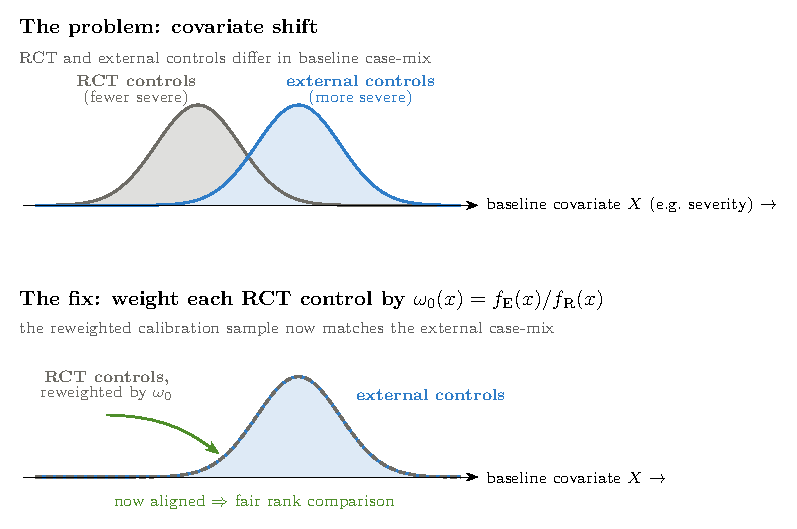
\includegraphics[width=0.86\linewidth]{fig_shift.pdf}
\caption{Covariate shift and its correction. \emph{Top:} randomized and external controls may carry different baseline case-mix, so the covariate densities $f_{\R}$ and $f_{\E,0}$ differ even when the compatible external control-outcome law is identical given $X$. \emph{Bottom:} weighting each randomized control by the density ratio $\omega_0(x)=f_{\E,0}(x)/f_{\R}(x)$ makes the calibration sample represent the external case-mix, so conformal ranks stay calibrated despite the shift. Unweighted ranks would instead flag high-severity compatible external controls as extreme purely because such subjects are over-represented externally---the failure mode this weighting removes.}
\label{fig:shift}
\end{figure}

For an oracle derivation, define the null/compatible density ratio
\[
\omega_0(x)=\frac{f_{\E,0}(x)}{f_{\R}(x)}.
\tag{10}
\]
If contamination is independent of $X$, then the compatible external covariate distribution equals the overall external covariate distribution and $\omega_0$ can be estimated using all external covariates. If the probability of incompatibility depends on $X$, the overall external ratio need not equal the null ratio; this is a major open issue and a required stress-test scenario.

\subsection{Step 6: explain weighted split calibration before introducing the CV implementation}

Let a score function be fixed after training. For randomized-control calibration scores $V_i^{\R}$ and one external score $V_j^{\E}$, define normalized masses
\[
\pi_i(x_j)
=
\frac{\omega_0(X_i^{\R})}
{\omega_0(X_j^{\E})+\sum_{\ell\in\mathcal C_1}\omega_0(X_\ell^{\R})},
\]
for calibration subjects, and
\[
\pi_j(x_j)
=
\frac{\omega_0(X_j^{\E})}
{\omega_0(X_j^{\E})+\sum_{\ell\in\mathcal C_1}\omega_0(X_\ell^{\R})}.
\]
A conservative upper-tail weighted split-conformal $p$-value is
\[
p_{j,\mathrm{split}}^{w}
=
\pi_j(x_j)
+
\sum_{i\in\mathcal C_1}\pi_i(x_j)
\ind(V_i^{\R}\ge V_j^{\E}).
\tag{11}
\]
This is the weighted analogue of equation (1). Under known density ratio, weighted exchangeability, and a fixed score, weighted conformal theory yields marginal super-uniformity under covariate shift \citep{tibshirani2019weighted,jin2026weighted}.

The population identity behind (11) is simple and important. Let
\[
G_x(v)=\Pr(V\le v\mid X=x,B=0).
\]
Then
\[
\begin{aligned}
\Exp_{\R}\{\omega_0(X)\ind(V\le v)\}
&=\int G_x(v)\frac{f_{\E,0}(x)}{f_{\R}(x)}f_{\R}(x)\,dx\\
&=\int G_x(v)f_{\E,0}(x)\,dx\\
&=\Pr_{\E,0}(V\le v).
\end{aligned}
\tag{12}
\]
Thus the weighted randomized-control score distribution represents the score distribution that compatible external controls would have under their own covariate mix.

\subsection{Step 7: use cross-validated conformal scores in the actual implementation}

A single split wastes randomized controls, which are often scarce. The intended implementation therefore uses $K$-fold cross-validation, following the CV+ idea used in CSB \citep{zhu2025csb,barber2021jackknife}.

\begin{figure}[ht]\centering
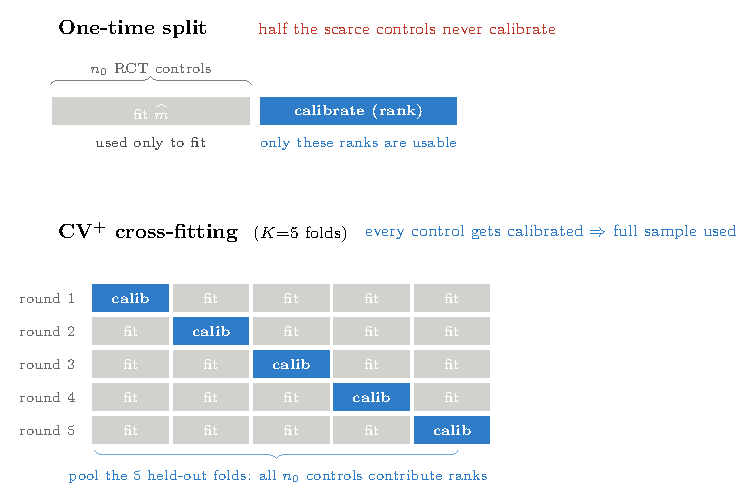
\includegraphics[width=0.84\linewidth]{fig_cv.pdf}
\caption{Why cross-fitting (CV$^+$) rather than a one-time split. \emph{Top:} a single train/calibrate split spends half of the scarce randomized controls on fitting the model and only calibrates ranks on the other half. \emph{Bottom:} $K$-fold cross-fitting scores each fold from a model fit on the remaining folds, so every randomized control eventually contributes a calibration rank; pooling the held-out folds uses the whole control sample. This is the main efficiency lever behind sym-ada's power gain (Table~\ref{tab:refcell}).}
\label{fig:cv}
\end{figure}

For each randomized control $i\in\mathcal C_k$, compute an out-of-fold score
\[
V_i
=s\{\bm Y_i,X_i;\widehat\eta^{(-k)}\}.
\]
For each external subject $j$, evaluate it under the corresponding fold-specific model:
\[
V_j^{(-k)}
=s\{\bm Y_j,X_j;\widehat\eta^{(-k)}\}.
\]
A natural proposed weighted CV rank statistic is
\[
\widehat p_{j,\mathrm{CV}}^{w}
=
\frac{
\widehat\omega(X_j)
+
\sum_{k=1}^{K}\sum_{i\in\mathcal C_k}
\widehat\omega(X_i)
\ind\{V_i\ge V_j^{(-k)}\}
}
{
\widehat\omega(X_j)
+
\sum_{i\in\mathcal C}\widehat\omega(X_i)
}.
\tag{13}
\]
This uses every randomized control for out-of-fold calibration while preventing a subject from being evaluated by a model trained on itself.

Equation (13) is the intended working implementation, but its theoretical status must be stated honestly. The ordinary unweighted CSB CV+ construction has a conservative finite-sample bound rather than the exact split-conformal $\gamma$ bound \citep{zhu2025csb}. A weighted CV+ theorem for the proposed longitudinal score does not follow automatically from the split result and is a central theoretical task. Simulations should therefore include:
\begin{itemize}
    \item oracle weighted split conformal as a validity benchmark;
    \item the practical weighted CV statistic (13);
    \item optionally, a guaranteed but conservative aggregation of fold-specific weighted split $p$-values.
\end{itemize}

\subsection{Step 8: screen conservatively}\label{sec:screen}

For a signed score $V_j=c^{\top}\bm r_j$ standardized as in Step~3, the upper-tail weighted $p$-value $\widehat p_{j,\mathrm{hi}}^{w}$ is exactly (13); it is small when the external trajectory sits unusually \emph{high}. The base one-sided screen retains
\[
\widehat{\mathcal E}_{\gamma}
=
\{j:\widehat p_{j,\mathrm{hi}}^{w}>\gamma\}.
\tag{14}
\]
This threshold is a conservative compatibility screen, not a prediction-interval exclusion rate; because weighted $p$-values have nonuniform discrete support in $X$, ``larger than every internal residual'' is useful intuition but not the formal weighted rule. Beyond $\gamma$ the screen has two design choices---its \emph{orientation} and whether $\gamma$ is fixed or \emph{adaptive}---defined next.

\paragraph{Two tails from one fit.} The complementary lower-tail $p$-value is the upper-tail statistic applied to the negated score, i.e.\ (13) with $\ind\{V_i\ge V_j^{(-k)}\}$ replaced by $\ind\{V_i\le V_j^{(-k)}\}$:
\[
\widehat p_{j,\mathrm{lo}}^{w}
=
\frac{\widehat\omega(X_j)+\sum_{k=1}^{K}\sum_{i\in\mathcal C_k}\widehat\omega(X_i)\ind\{V_i\le V_j^{(-k)}\}}
{\widehat\omega(X_j)+\sum_{i\in\mathcal C}\widehat\omega(X_i)},
\]
small when the trajectory sits unusually \emph{low}. Both tails come from the same fold-specific fits, so no extra model fitting is required.

\paragraph{Symmetric two-sided screen.} Score by the folded contrast $|V_j|=|c^{\top}\bm r_j|$, apply (13) to $|V|$, and retain $\{j:\widehat p_{j,|V|}^{w}>\gamma\}$ with a \emph{single} threshold. This trims both tails equally. When the retained ECs are clean, $V$ is approximately symmetric about $0$, so equal trimming leaves the retained-score mean unchanged and the borrowed control mean unbiased; the cost is that half the deletion budget falls on the tail \emph{opposite} any directional contamination, lowering detection of it.

\paragraph{Non-symmetric two-sided screen.} Keep the signed score and use the two tail $p$-values with \emph{separate} thresholds $\gamma_{\mathrm{hi}},\gamma_{\mathrm{lo}}$:
\[
\widehat{\mathcal E}_{\gamma_{\mathrm{hi}},\gamma_{\mathrm{lo}}}^{\mathrm{ns}}
=
\bigl\{j:\ \widehat p_{j,\mathrm{hi}}^{w}>\gamma_{\mathrm{hi}}\ \text{and}\ \widehat p_{j,\mathrm{lo}}^{w}>\gamma_{\mathrm{lo}}\bigr\},
\]
i.e.\ EC $j$ is deleted iff $\widehat p_{j,\mathrm{hi}}^{w}\le\gamma_{\mathrm{hi}}$ or $\widehat p_{j,\mathrm{lo}}^{w}\le\gamma_{\mathrm{lo}}$. Cutting the high tail hard ($\gamma_{\mathrm{hi}}$) and the low tail lightly ($\gamma_{\mathrm{lo}}$) targets a positive-shift contamination while keeping a light lower cut. Two special cases recover the others: $\gamma_{\mathrm{lo}}{=}0$ is the one-sided screen (14), and $\gamma_{\mathrm{hi}}{=}\gamma_{\mathrm{lo}}$ is the signed-tail analogue of the symmetric screen.

\paragraph{The orientation bias.} Selecting on the same contrast used for the estimand induces a truncation bias in the borrowed mean. Write $Z=c^{\top}\bm Y=c^{\top}\widehat m(X)+\widehat s(X)\,V$, so within a stratum $Z$ is affine in the score $V$ with standardizing scale $\widehat s(X)$. Deleting the top $\gamma_{\mathrm{hi}}$ and bottom $\gamma_{\mathrm{lo}}$ of a clean, symmetric $V$ shifts the retained mean by
\[
\Exp\bigl[Z\mid\text{retained, clean}\bigr]-\Exp[Z\mid\text{clean}]
\;\approx\;-\,\widehat s(X)\,\bigl\{q(\gamma_{\mathrm{hi}})-q(\gamma_{\mathrm{lo}})\bigr\},
\]
where $q(\cdot)$ is the tail-mean contribution of the trimmed fraction; the shift is negative and monotone in the asymmetry $\gamma_{\mathrm{hi}}-\gamma_{\mathrm{lo}}$. A lower borrowed control mean $\widehat\mu_0$ raises $\widehat\tau=\widehat\mu_1-\widehat\mu_0$, so the estimator carries a positive bias proportional to $\gamma_{\mathrm{hi}}-\gamma_{\mathrm{lo}}$: zero for the symmetric screen, small for a mild asymmetry, large for an aggressive one-sided cut. The oracle screen avoids it because it deletes by the outcome-independent contamination label and never trims clean ECs; a soft-borrowing variant that removes the bias \emph{without} reverting to symmetry is left to future work.

\begin{figure}[ht]\centering
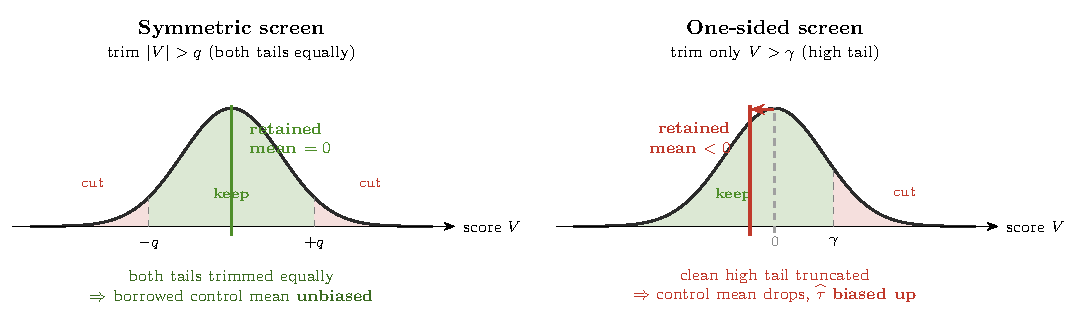
\includegraphics[width=0.98\linewidth]{fig_trimming.pdf}
\caption{The orientation bias, visualized. On a clean external-control set the score $V=c^{\top}\bm r$ is approximately symmetric about $0$. \emph{Left (symmetric screen):} trimming $|V|>q$ removes both tails equally, so the retained-score mean stays at $0$ and the borrowed control mean $\widehat\mu_0$---hence $\widehat\tau$---is unbiased. \emph{Right (one-sided/non-symmetric screen):} cutting only the high tail $V>\gamma$ truncates the clean upper tail, shifts the retained mean below $0$, lowers $\widehat\mu_0$, and biases $\widehat\tau$ upward by an amount that grows with the asymmetry $\gamma_{\mathrm{hi}}-\gamma_{\mathrm{lo}}$. This is the mechanism behind the non-symmetric screens' apparent power in Table~\ref{tab:refcell}: it is bias and type-I inflation, not valid signal.}
\label{fig:trimming}
\end{figure}

\paragraph{Adaptive threshold.} Rather than fix the thresholds, choose them per dataset to minimize an estimated mean-squared error of the borrowing estimate. On a grid $\mathcal G$ of $(\gamma_{\mathrm{hi}},\gamma_{\mathrm{lo}})$ pairs (a one-dimensional grid of $\gamma$ for the symmetric screen), let $\widehat\tau(\gamma)$ be the screened borrowing estimate and $\widehat\tau_{\mathrm{RCT}}$ the no-borrow estimate, and set
\[
\widehat{\mathrm{MSE}}(\gamma)
=
\underbrace{\max\!\bigl[\bigl\{\widehat\tau(\gamma)-\widehat\tau_{\mathrm{RCT}}\bigr\}^2-\widehat{\mathrm{Var}}^{\ast}\!\bigl\{\widehat\tau(\gamma)-\widehat\tau_{\mathrm{RCT}}\bigr\},\ 0\bigr]}_{\text{de-biased squared bias (CSB)}}
+
\underbrace{\widehat{\mathrm{Var}}^{\ast}\bigl\{\widehat\tau(\gamma)\bigr\}}_{\text{bootstrap variance}},
\qquad
\gamma^{\ast}=\arg\min_{\gamma\in\mathcal G}\widehat{\mathrm{MSE}}(\gamma),
\]
reporting $\widehat\tau(\gamma^{\ast})$. Because the randomized-control estimate is unbiased by design, $\{\widehat\tau(\gamma)-\widehat\tau_{\mathrm{RCT}}\}^2$ is a label-free plug-in for the squared borrowing bias, and $\widehat{\mathrm{Var}}^{\ast}$ is taken across the full-pipeline bootstrap that re-screens each resample. This is the adaptive-selection principle of CSB \citep{zhu2025csb}, in its de-biased form: the raw plug-in $\{\widehat\tau(\gamma)-\widehat\tau_{\mathrm{RCT}}\}^2$ also contains $\mathrm{Var}\{\widehat\tau(\gamma)-\widehat\tau_{\mathrm{RCT}}\}$ and so overstates the bias, so we subtract the \emph{paired} bootstrap variance of that difference (floored at $0$), leaving an approximately unbiased squared-bias estimate; both variances are taken across the full-pipeline bootstrap that re-screens each resample. One honest caveat remains: because $\gamma^{\ast}$ is selected on the point estimate and then reused inside the bootstrap interval, coverage is only empirically, not provably, controlled (a nested bootstrap would be needed for a formal guarantee). A fixed $\gamma=0.10$ with a sensitivity grid remains a conservative default; the adaptive rule prevents the aggressive-cut trap in which a large $\gamma_{\mathrm{hi}}$ inflates apparent power through the orientation bias above.

\subsection{Step 9: refit the final borrowing estimator after screening}\label{sec:refit}

Screening and estimation use different weights and opposite transport directions.

The screening ratio is approximately
\[
\omega_0(x)=\frac{f_{\E,0}(x)}{f_{\R}(x)},
\]
which makes randomized calibration scores represent compatible external covariates.

After selection, the final EC-to-RCT transport ratio is
\[
\rho_{\gamma}(x)
=
\frac{f_{\R}(x)}{f_{\E,\gamma}(x)},
\]
where $f_{\E,\gamma}$ is the covariate distribution among retained external controls. It must be re-estimated using the retained sample.

For the scalar longitudinal contrast
\[
Z=c^{\top}\bm Y,
\]
a generic transported augmented estimator of the untreated trial mean is
\[
\widehat\mu_{0,\gamma}^{\E,\mathrm{DR}}
=
\frac{1}{n_{\R}}\sum_{i:S_i=1}\widehat m_{0,\gamma}(X_i)
+
\frac{
\sum_{j:S_j=0,\,j\in\widehat{\mathcal E}_{\gamma}}
\widehat\rho_{\gamma}(X_j)
\{Z_j-\widehat m_{0,\gamma}(X_j)\}
}
{
\sum_{j:S_j=0,\,j\in\widehat{\mathcal E}_{\gamma}}
\widehat\rho_{\gamma}(X_j)
}.
\tag{15}
\]
This external estimate can be combined with the randomized-control estimate through the second-layer borrowing weight used in the JRSS-A framework \citep{zhou2025causal}. The treated mean is estimated from randomized treated subjects, and the final estimate is
\[
\widehat\tau_{c,\gamma}
=
\widehat\mu_{1,c}^{\R}
-
\left\{(1-\lambda_\gamma)\widehat\mu_{0,c}^{\R}
+\lambda_\gamma\widehat\mu_{0,\gamma}^{\E,\mathrm{DR}}\right\}.
\tag{16}
\]
All source, outcome, variance, and optimal-borrowing components used in (15)--(16) are refitted after screening; in particular the retained-source density $f_{\E,\gamma}$ in $\widehat\rho_\gamma$ is re-estimated on the retained external controls, not carried over from the pre-screening fit.

\paragraph{Two implementation choices relative to the reference frameworks.} The borrowing weight $\lambda_\gamma$ in (16) is the efficient inverse-variance weight $\widehat V_{\R}/(\widehat V_{\R}+\widehat V_{\E,\gamma})$ with the \emph{estimated} control-mean variances plugged in. This coincides with the homoscedastic JRSS-A weight of \citet{zhou2025causal} when the randomized and external controls share a residual variance, but improves on it when the external controls are noisier---it then borrows less and lowers RMSE---so we keep this outcome-aware form rather than the unit-variance simplification. The adaptive threshold in (14) uses the CSB \emph{de-biased} objective of \citet{zhu2025csb} (the paired-variance subtraction above), matching that reference rather than the raw plug-in. Neither choice reorders the screens head-to-head; the borrowing-weight choice is visible only at the \emph{full}-borrow anchor, where the outcome-aware weight down-weights the contamination-inflated external variance (so full EC-AIPW there looks less catastrophic than a unit-variance weight would make it).

The construction is clear, but post-selection consistency and variance inference are not automatic. They remain methodological questions to be studied by theory and by resampling the entire pipeline.

\section{Unified toy longitudinal model and simulation design}

This section combines the analytically tractable toy example and the full simulation protocol. It does not use SUNFISH-calibrated parameters. The goal is to isolate mechanisms before moving to a realistic application.

\subsection{Design at a glance}

This study uses \emph{three} data-generating processes (Section~\ref{sec:dgps}) of increasing departure from a simple toy: (1)~the \emph{base binary} DGP---one binary severity covariate, severity-dependent variance---which is analytically tractable and drives the reference cell and every early result; (2)~a \emph{homoscedastic} variant that decouples the variance from the covariate; and (3)~a \emph{two-covariate} DGP---one binary, one continuous, covariate-free variance---that removes the binary-stratum structure entirely. The first is primary; the other two are robustness/generalization stress tests.

Held fixed across the study: $n_{\R,1}=120$, $n_{\R,0}=60$, $n_{\E}=200$, $X$-independent contamination, and a correctly specified (or, for DGP~3, estimated) density ratio. The broad diagnostic sweep fixes $\pi_B=0.5$ and $\gamma=0.10$; the estimation \emph{reference cell} (Section~\ref{sec:basecell}) uses $\pi_B=0.3$ with adaptive $\gamma$. The varied axes:

\emph{Screening axes} (diagnostic, on the base DGP):
\begin{itemize}
    \item score shape --- quadratic / max / contrast-$c_1$ / contrast-$c_2$
    \item covariance --- raw / internal / source-specific
    \item weighting --- weighted ($\omega_0$) / unweighted
    \item calibration --- one-time split / $K{=}5$ CV+
    \item working model --- correct / moderate / severe
    \item drift pattern --- A global / B late / C slope / D severity-specific
    \item drift magnitude $\Delta$ --- $0$ (null) / $1$ / $3$ / $5$ / $8$ (large, near-separable)
\end{itemize}

\emph{Estimation adds:}
\begin{itemize}
    \item estimand --- $c_1$ (final$-$baseline) / $c_2$ (average)
    \item final method --- RCT-only / full EC-AIPW / oracle (delete exactly the contaminated) / screened$+$AIPW
    \item screen orientation \& threshold --- symmetric vs.\ non-symmetric two-sided; fixed vs.\ adaptive $\gamma$ (both defined in Step~8, Section~\ref{sec:screen})
    \item contamination fraction --- $\pi_B\in\{0.15,0.30,0.50\}$
\end{itemize}

\paragraph{Core questions and the comparison that answers each.} The method's value lives at $\Delta>0$. Each question names the single comparison (axis $\times$ metric) that isolates it.

\emph{Calibration and specificity.}
\begin{enumerate}
    \item \textbf{Null specificity} --- does the screen leave compatible ECs alone? At $\Delta{=}0$: false-exclusion rate vs.\ the target $\gamma$, across working models.
    \item \textbf{Does weighting repair covariate-shift miscalibration, and by which mechanism?} Weighted vs.\ unweighted false-exclusion. The miscalibration is \emph{variance-driven} in the base DGP (present even under a correct model) but \emph{misspecification-driven} in DGPs~2--3 (present only when a shifted covariate is omitted).
    \item \textbf{Robustness to outcome-model misspecification} --- false-exclusion and detection across correct / moderate / severe working models.
\end{enumerate}

\emph{Detection and estimand alignment.}
\begin{enumerate}\setcounter{enumi}{3}
    \item \textbf{Which score catches which drift, and is detection estimand-aligned?} Detection by score shape $\times$ drift pattern A--D at $\Delta{=}3$ (e.g.\ $c_1$ is blind to the global shift A, which is orthogonal to it; $c_2$ misses shape drift that averages out).
    \item \textbf{Is the detection ceiling estimation noise or intrinsic overlap?} Detection with estimated vs.\ oracle (true mean and variance) nuisances; if it barely moves, the limit is overlap, not estimation.
    \item \textbf{Detection vs.\ signal} --- detection over $\Delta\in\{1,3,5,8\}$ and the severe-stratum signal-to-noise floor.
\end{enumerate}

\emph{Estimation.}
\begin{enumerate}\setcounter{enumi}{6}
    \item \textbf{Does screening cut borrowing bias and restore coverage vs.\ full borrow?} Bias and $95\%$ coverage for RCT-only / full-EC / oracle / screened at $\Delta>0$.
    \item \textbf{Non-symmetric $+$ adaptive $\gamma$ vs.\ symmetric vs.\ fixed one-sided} --- does it gain power while controlling the selection bias? Bias / type-I / power across the four screens at the reference cell.
    \item \textbf{Does borrowing beat RCT-only, and in which regime?} Power and RMSE of sym-ada vs.\ RCT-only vs.\ oracle across noise level (base vs.\ homoscedastic DGP) and $\pi_B$.
\end{enumerate}

\emph{Robustness and generalization.}
\begin{enumerate}\setcounter{enumi}{9}
    \item \textbf{Does the method survive without the binary-stratum structure?} On DGP~3: whether the continuous density-ratio weighting (oracle vs.\ logistic) restores false-exclusion control under severe misspecification, and whether the general AIPW preserves the sym-ada-beats-RCT conclusion.
    \item \textbf{Covariance treatment and its fragility} --- raw / internal / source false-exclusion and detection; the internal treatment is fragile to a between-source variance gap.
\end{enumerate}

\emph{Deferred} (later work): $X$-dependent contamination; a covariate-driven (plasmode) DGP calibrated to real data.

\subsection{Base scenario: the reference cell}\label{sec:basecell}

Every estimation comparison is read against a single reference cell, at which the \emph{borrowing methods are compared head-to-head} and every other run is exactly one axis away. The cell fixes: the base binary DGP (eq.~(17)--(22)) with $\sigma(X){=}(1,1.8)$; contamination fraction $\pi_B{=}0.3$ (a realistic operating point at which borrowing can pay); drift pattern~A (global shift) at $\Delta{=}8$ (a signal-to-noise level at which the contamination is detectable, so that borrowing can help without net bias); estimand $c_2$ (visit average, $\tau_{c_2}{=}0.4625$); weighted CV+ rank calibration; correct working model. Table~\ref{tab:refcell} compares the methods, varying \emph{one nonconformity-score axis at a time} from the default screen (contrast-$c_2$, internal covariance, symmetric adaptive $\gamma$): three anchors (RCT-only, full EC-AIPW, oracle); the \emph{score shape} (quadratic Mahalanobis / max worst-visit); the \emph{residual standardization} (raw / internal / source-specific covariance); and, for the contrast, the \emph{orientation} (symmetric adaptive \textbf{sym-ada}; fixed aggressive \textbf{nonsym-fix}, $\gamma_{\mathrm{hi}}{=}0.30,\gamma_{\mathrm{lo}}{=}0.05$; non-symmetric adaptive \textbf{nonsym-ada}, Step~8). The rest of the section then moves the DGP/scenario axes one at a time away from this setting.

\begin{table}[ht]
\centering
\caption{Reference cell --- borrowing methods compared at one fixed setting ($\pi_B{=}0.3$, pattern~A, $\Delta{=}8$, estimand $c_2$, $\tau_{c_2}{=}0.4625$; weighted \textbf{CV+} rank calibration, correct model; $n_{\E}{=}200$, $300$ replicates, $B{=}500$ full-pipeline bootstraps; borrowing weight $\lambda$ = efficient inverse-variance, adaptive $\gamma$ = de-biased CSB). Each block varies one nonconformity-score axis from the default (contrast-$c_2$, internal covariance, \textbf{sym-ada}). sym-ada is the only \emph{attainable} method that beats RCT-only on all four criteria at once: unbiased ($0.00$), lower RMSE ($0.18$ vs.\ $0.20$), type-I no worse than RCT-only ($0.06$), and higher power ($0.73$ vs.\ $0.64$); only the unattainable oracle does better. Cross-validated (CV+) calibration instead of a one-time split lifts sym-ada's power from $0.65$ to $0.73$ by calibrating on the whole randomized-control sample. The non-symmetric screens buy more raw power (nonsym-ada $0.84$, nonsym-fix $0.99$) only by paying bias ($+0.05$, $+0.31$) and inflated type-I ($0.08$, $0.31$), so that extra power is not valid inference.}
\begin{tabular}{lcccccc}
\toprule
Method & Detection & False-excl. & Bias & RMSE & Type-I & Power \\
\midrule
\multicolumn{7}{@{}l}{\emph{Anchors}} \\
RCT-only                & --- & --- & $-0.00$ & $0.20$ & $0.06$ & $0.64$ \\
Full EC-AIPW            & --- & --- & $-0.42$ & $0.49$ & $0.42$ & $0.06$ \\
Oracle                  & $1.00$ & $0.00$ & $-0.00$ & $0.17$ & $0.06$ & $0.75$ \\
\midrule
\multicolumn{7}{@{}l}{\emph{Score shape} (internal cov, adaptive $\gamma$)} \\
quadratic (Mahalanobis) & $0.99$ & $0.18$ & $-0.01$ & $0.18$ & $0.04$ & $0.70$ \\
max (worst visit)       & $0.97$ & $0.07$ & $+0.07$ & $0.21$ & $0.09$ & $0.88$ \\
\midrule
\multicolumn{7}{@{}l}{\emph{Residual standardization} (contrast-$c_2$, non-symmetric adaptive $\gamma$)} \\
raw covariance          & $0.99$ & $0.07$ & $+0.04$ & $0.20$ & $0.07$ & $0.80$ \\
source-specific         & $0.98$ & $0.00$ & $-0.01$ & $0.18$ & $0.06$ & $0.72$ \\
\midrule
\multicolumn{7}{@{}l}{\emph{Orientation} (contrast-$c_2$, internal cov) --- the non-symmetric comparators} \\
nonsym-fix ($\gamma_{\mathrm{hi}}{=}0.30$) & $1.00$ & $0.32$ & $+0.31$ & $0.36$ & $0.31$ & $0.99$ \\
nonsym-ada              & $0.99$ & $0.07$ & $+0.05$ & $0.20$ & $0.08$ & $0.84$ \\
\midrule
\multicolumn{7}{@{}l}{\emph{Reference default}} \\
\textbf{contrast-$c_2$, internal, sym-ada} & $1.00$ & $0.10$ & $0.00$ & $\mathbf{0.18}$ & $0.06$ & $\mathbf{0.73}$ \\
\bottomrule
\end{tabular}
\label{tab:refcell}
\end{table}

\begin{figure}[ht]
\centering

\includegraphics[width=\linewidth]{fig_outcome.pdf}\\[2pt]
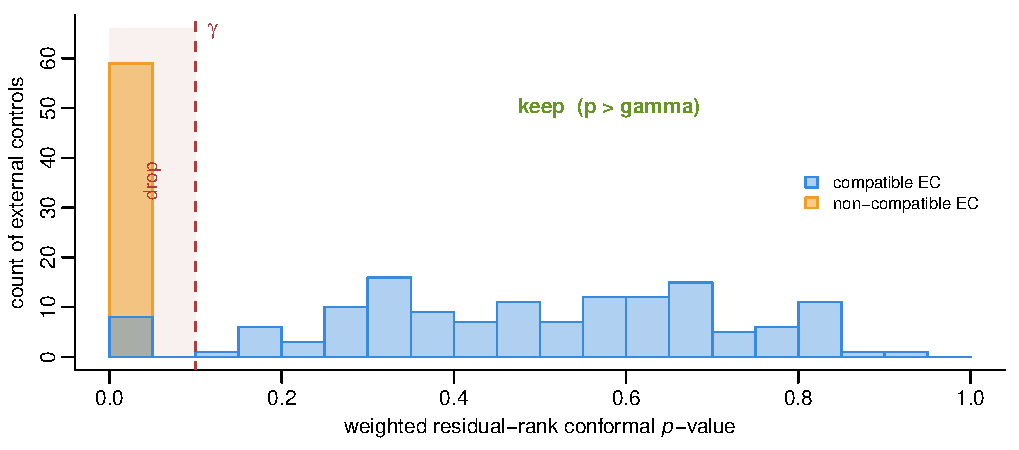
\includegraphics[width=\linewidth]{fig_pval.pdf}
\caption{The screen on the reference-cell setup ($n_{\R,0}{=}60$, $n_{\E}{=}200$, $\pi_B{=}0.3$, $\Delta{=}8$, contrast-$c_2$, weighted CV+ calibration; one real simulation draw). \emph{Top:} density of the visit-average control outcome $Z=c_2^{\top}\bm Y$. Compatible external controls (blue) overlap the randomized controls (gray) but sit slightly higher \emph{purely because the external mix carries more severe subjects} (covariate shift), not because they are incompatible; contaminated external controls (amber) sit far right. A raw-outcome threshold would confound covariate shift with contamination. \emph{Bottom:} the weighted residual-rank conformal $p$-values. Contaminated ECs pile up near $p{=}0$ and fall below the threshold $\gamma$---all screened out---while compatible ECs are roughly uniform on $(0,1]$ and kept; only about $6\%$ fall below $\gamma$ (the false-exclusion rate). The screen is thus a truncation of the calibrated $p$-value scale at $\gamma$, not a cutoff on the raw outcome.}
\label{fig:screen-mechanism}
\end{figure}

\begin{figure}[ht]\centering
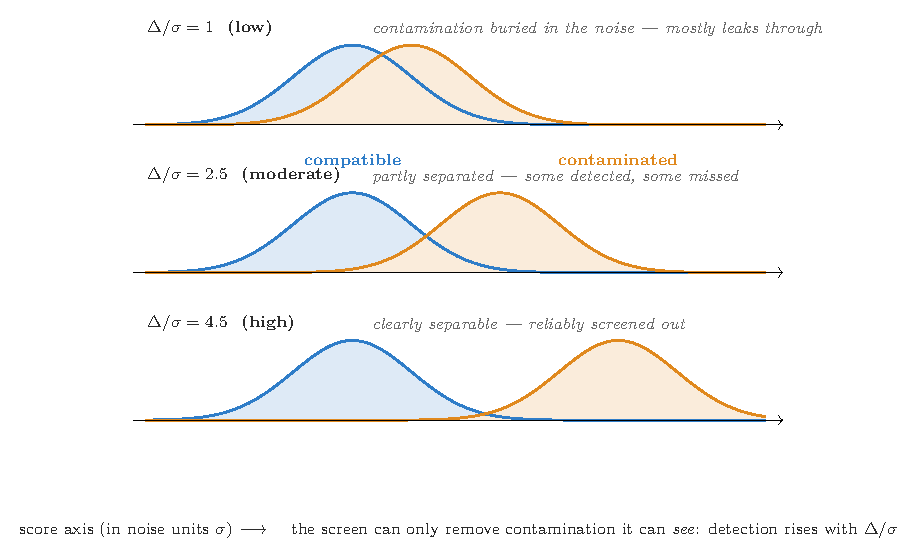
\includegraphics[width=0.9\linewidth]{fig_snr.pdf}
\caption{The signal-to-noise limit on detection. As the contamination magnitude $\Delta$ grows relative to the residual noise $\sigma$, the contaminated external-control score distribution (amber) separates from the compatible one (blue). At low $\Delta/\sigma$ the two overlap and contamination is largely undetectable---it leaks through any screen; at high $\Delta/\sigma$ it is cleanly separable and reliably removed. The screen can only delete contamination it can \emph{see}, so detection---and hence the safety of borrowing---depends on the drift's signal-to-noise ratio: borrowing is safest precisely when incompatibility is either absent or large enough to catch, and residual undetected drift at low $\Delta/\sigma$ is the method's main limitation.}
\label{fig:snr}
\end{figure}

\subsection{Data-generating processes}\label{sec:dgps}

The study uses three processes of increasing departure from the toy; the first is primary, the other two probe robustness and generalization (core questions~2, 9, 10, 11).

\subsubsection{DGP 1: base binary process (heteroscedastic)}

Use four visits
\[
t\in\{0,1,2,3\}
\]
and one binary baseline severity covariate $X$.

Randomized and external covariate distributions differ:
\[
X\mid S=1\sim\mathrm{Bernoulli}(0.30),
\qquad
X\mid S=0\sim\mathrm{Bernoulli}(0.70).
\tag{17}
\]
This creates covariate shift but preserves overlap.

For every randomized or compatible external control, generate the untreated trajectory
\[
Y_t(0)
=
2+0.5t+X(1+0.4t)+b+\sigma(X)\varepsilon_t,
\tag{18}
\]
where
\[
b\sim N(0,0.5^2),
\qquad
\bm\varepsilon\sim N_4(\bm 0,R),
\qquad
R_{uv}=0.5^{|u-v|},
\]
and
\[
\sigma(0)=1,
\qquad
\sigma(1)=1.8.
\tag{19}
\]
Thus severe subjects have a different mean trajectory and greater residual variability.

For randomized treated subjects, add a treatment-effect trajectory
\[
\bm\tau=(0,0.25,0.60,1.00)^{\top},
\qquad
\bm Y(1)=\bm Y(0)+\bm\tau.
\tag{20}
\]
Two estimands are studied, chosen so that a given drift projects onto them differently:
\[
c_1=(-1,0,0,1)^{\top}\ (\text{final minus baseline}),
\qquad
c_2=(\tfrac14,\tfrac14,\tfrac14,\tfrac14)^{\top}\ (\text{visit average}),
\tag{21}
\]
with true effects $\tau_{c_1}=c_1^{\top}\bm\tau=1.000$ and $\tau_{c_2}=c_2^{\top}\bm\tau=0.4625$. The random intercept $b$ cancels in $c_1$ (because $c_1^{\top}\bm 1=0$) but not in $c_2$, so the two contrasts have different residual scales and signal-to-noise, and the same drift can bias one while leaving the other unaffected.

Sample sizes are
\[
n_{\R,1}=120,
\qquad
n_{\R,0}=60,
\qquad
n_{\E}=200.
\tag{22}
\]
The practical screen uses $K=5$-fold CV+; a one-time sample split is included as a finite-sample-valid comparison.

\paragraph{Variance-structure variants.}
The base DGP makes the residual scale severity-dependent, $\sigma(0){=}1$, $\sigma(1){=}1.8$, and equal across sources. Two one-component variants probe the covariance machinery: (i) \emph{homoscedastic}, $\sigma{\equiv}1$ for all subjects and both sources ($X$-independent); (ii) \emph{source-different}, $\sigma_{\R}{\equiv}1$ for randomized controls but $\sigma_{\E}{\equiv}1.8$ for external controls ($X$-independent). Variant (ii) is the pointed stress: the internal-covariance screen standardizes external scores by the randomized-control covariance, so a genuine between-source variance gap is mis-standardized. Both leave the estimand $\tau_{c_2}{=}0.4625$ unchanged.

\subsubsection{Why ordinary ranks fail under covariate shift (base DGP)}

For any fixed fitted score, write
\[
G_0(v)=\Pr(V\le v\mid X=0,B=0),
\qquad
G_1(v)=\Pr(V\le v\mid X=1,B=0).
\]
The randomized-control marginal score distribution is
\[
F_{\R}(v)=0.70G_0(v)+0.30G_1(v),
\tag{23}
\]
while the compatible external marginal is
\[
F_{\E,0}(v)=0.30G_0(v)+0.70G_1(v).
\tag{24}
\]
If the raw or inadequately standardized score has different distributions across severity groups, $G_0\neq G_1$, then $F_{\R}\neq F_{\E,0}$ even though the conditional outcome law is identical across sources.

For the simple unweighted maximum-only rule with $n_C$ randomized calibration subjects, the false-exclusion probability for one compatible external subject is
\[
\Pr\left(V^{\E}>\max_{1\le i\le n_C}V_i^{\R}\right)
=
\int F_{\R}(v)^{n_C}\,dF_{\E,0}(v).
\tag{25}
\]
Only when $F_{\R}=F_{\E,0}$ does this equal $1/(n_C+1)$. Equation (25) provides a direct mathematical target for the simulation.

Under oracle weighting,
\[
\omega_0(0)=\frac{0.30}{0.70},
\qquad
\omega_0(1)=\frac{0.70}{0.30},
\tag{26}
\]
and the weighted randomized mixture becomes
\[
F_{\R}^{w}(v)
=0.30G_0(v)+0.70G_1(v)
=F_{\E,0}(v).
\tag{27}
\]
This equality holds even if the working longitudinal mean model is misspecified, because the same misspecification is contained inside both $G_0$ and $G_1$.

\subsubsection{DGP 2: homoscedastic (variance decoupled from the covariate)}

A one-change variant of DGP~1 makes the residual scale covariate-free, $\sigma(X){\equiv}\sigma$ with $\sigma{=}1$, keeping the single binary $X$, the mean (18), and everything else. The residual covariance $\Sigma=0.25\,\bm 1\bm 1^{\top}+\sigma^2 R$ is then a \emph{single} $4\times4$ matrix, so the per-stratum covariance and its fragility disappear by construction. A companion \emph{source-different} case keeps the variance covariate-free but unequal across sources, $\sigma_{\R}{\equiv}1$, $\sigma_{\E}{\equiv}1.8$, to stress the internal-covariance assumption (a between-source variance gap). This DGP isolates a distinct point: with the variance decoupled from $X$, a correct working model leaves covariate-free residuals, so unweighted ranks are already calibrated and the covariate-shift miscalibration becomes \emph{misspecification-driven} rather than variance-driven (contrast DGP~1).

\subsubsection{DGP 3: two covariates and homoscedastic variance}\label{sec:dgp2}

DGPs~1--2 lean on a single binary covariate: the per-stratum weights and the stratum-collapsed transport estimator exploit two cells. DGP~3 removes that structure entirely and is deliberately \emph{very} different.

\paragraph{Two covariates.} Each subject carries a binary severity covariate $X_b$ and a continuous covariate $X_c$ (e.g.\ a baseline biomarker); both shift between sources:
\[
X_b\mid S{=}1\sim\mathrm{Bernoulli}(0.30),\quad X_b\mid S{=}0\sim\mathrm{Bernoulli}(0.70);
\qquad
X_c\mid S{=}1\sim N(0,1),\quad X_c\mid S{=}0\sim N(0.6,1).
\]
The continuous shift is moderate (mean gap $0.6$) to preserve overlap; extreme density-ratio weights are clipped.

\paragraph{Homoscedastic variance.} The residual scale does not depend on any covariate:
\[
Y_t(0)=2+0.5t+X_b(1+0.4t)+X_c(0.7+0.3t)+b+\sigma\,\varepsilon_t,
\qquad
b\sim N(0,0.5^2),\ \bm\varepsilon\sim N_4(\bm 0,R),\ \sigma=1,
\]
so $\Sigma=0.25\,\bm 1\bm 1^{\top}+\sigma^2 R$ is a \emph{single} $4\times4$ matrix, estimated once. As in DGP~2 this removes the per-stratum covariance machinery by construction, so the continuous covariate complicates only the \emph{weighting} and the \emph{estimator}, not the scoring. Treatment effect $\bm\tau$, estimands $c_1,c_2$, and contamination patterns A--D are unchanged.

\paragraph{Complementary miscalibration mechanism.} Under a correct mean model the residual is $b+\sigma\varepsilon$, covariate-free, so unweighted ranks are already calibrated; the miscalibration appears only under \emph{misspecification}, when the residual retains a shifted covariate. Together with DGP~1 (variance-driven) this shows weighting repairs both mechanisms.

\paragraph{Misspecification ladder for two covariates.} Redefined so all three levels stay genuinely distinct:
\begin{itemize}
    \item \emph{correct}: time, $X_b$, $X_c$, and both covariate$\times$time interactions;
    \item \emph{moderate}: omit both $\times$time interactions (residual retains the time-varying part of each covariate effect);
    \item \emph{severe}: additionally omit $X_c$ entirely (residual retains $(0.7+0.3t)X_c$). Because $X_c$ is shifted between sources, this is the case in which the \emph{continuous} density-ratio weighting must restore calibration.
\end{itemize}

\paragraph{Density ratio: now a genuine estimand.} With one binary covariate the logistic source model is saturated and oracle and estimated weights coincide. With $(X_b,X_c)$ the null density ratio $\omega_0(x)=f_{\E,0}(x)/f_{\R}(x)$ is a genuine function, with a closed form under the stated laws (a Bernoulli ratio times a Gaussian ratio) as an oracle benchmark, while the practical weight is estimated by a logistic source model $\Pr(S{=}0\mid X_b,X_c)$. This is exactly the density-ratio-estimation study the binary toy deferred; its estimation error and weight-clipping effect become measurable.

\paragraph{Estimator: the general transported AIPW.} The stratum-collapsed estimator does not apply. This DGP uses the general doubly robust estimator of Step~9 (Section~\ref{sec:refit}): an outcome regression $\widehat m_0(X_b,X_c)$ for the control contrast, transported to the randomized covariate distribution through the continuous ratio and augmented by the weighted residuals of the retained ECs, then combined with the randomized-control estimate through the inverse-variance borrowing weight $\lambda$. The binary toy's per-stratum estimator is its augmentation-free, two-cell reduction.

\paragraph{What it tests.} Holding the screen fixed (single $\Sigma$, continuous $\omega$, symmetric two-sided, adaptive $\gamma$), the runs vary model quality $\times$ weighting $\times$ estimand and ask: does the continuous density-ratio weighting recover false-exclusion control under severe misspecification (where the omitted, shifted $X_c$ would otherwise miscalibrate the screen); and does the general AIPW preserve the reference-cell conclusion---sym-ada beats RCT-only when the randomized controls are noisy---once the binary-$X$ stratum structure is gone. An affirmative answer shows the method is not an artifact of the toy.

\subsection{Partial external drift}

Introduce an external incompatibility indicator $B\sim\mathrm{Bernoulli}(\pi_B)$ with a fixed contamination fraction $\pi_B=0.5$, independent of $X$. Compatible external subjects ($B=0$) follow (18). Incompatible subjects ($B=1$) follow one of the four drift patterns below, each scaled by a magnitude $\Delta$ that is the primary signal-to-noise knob:
\[
\Delta\in\{0,1,3,5,8\}
\qquad
(\Delta=0\text{ is the null: all ECs compatible};\ \Delta=8\text{ is large, near-separable}).
\tag{28}
\]

\paragraph{A. Global mean shift.}
\[
\bm Y_{\E}(0)=\bm Y_{\mathrm{base}}(0)+\Delta(1,1,1,1)^{\top}.
\tag{29}
\]

\paragraph{B. Late drift.}
\[
\bm Y_{\E}(0)=\bm Y_{\mathrm{base}}(0)+\Delta(0,0,0,1)^{\top}.
\tag{30}
\]

\paragraph{C. Slope drift.}
\[
\bm Y_{\E}(0)=\bm Y_{\mathrm{base}}(0)+\Delta(0,1/3,2/3,1)^{\top}.
\tag{31}
\]

\paragraph{D. Severity-specific drift.}
\[
\bm Y_{\E}(0)=\bm Y_{\mathrm{base}}(0)+\Delta X(0,1/3,2/3,1)^{\top}.
\tag{32}
\]

\subsection{Contamination mechanism and density-ratio estimation}

The toy fixes $\Pr(B=1\mid X)=\pi_B$ independent of $X$, so the covariate distribution of compatible ECs equals the overall external covariate distribution and a single correctly specified density ratio $\omega_0=f_{\E,0}/f_{\R}$ suffices. This isolates the weighting mechanism from density-ratio estimation error.

The complementary stress test---$X$-dependent contamination $\Pr(B=1\mid X)=\operatorname{expit}(\eta_0+\eta_1X)$, under which the estimable overall ratio $f_{\E}/f_{\R}$ diverges from the null ratio $\omega_0$---is deferred to a future edge-case study. With a single binary $X$ the logistic source model is saturated, so the alternative weight estimators (correctly specified vs.\ misspecified logistic source models, entropy balancing \citep{hainmueller2012}) coincide and cannot be separated; distinguishing them requires a continuous covariate, which the two-covariate DGP~3 (Section~\ref{sec:dgp2}) supplies.

\subsection{Working outcome-model specifications}

Use three levels of model quality.

\paragraph{Correct working mean model.}
Include time, $X$, and $X\times$time, with an adequate covariance model.

\paragraph{Moderate misspecification.}
Omit the $X\times$time interaction.

\paragraph{Severe misspecification.}
Use only time main effects or a linear time trend, omitting severity effects and nonlinear trajectory structure.

The key calibration question is whether compatible EC false-exclusion remains controlled under misspecification. The key power question is how much ability to detect (29)--(32) is lost when randomized-control residuals become noisy.

\subsection{Nonconformity scores: twelve variants}

The residual vector $\bm r=\bm Y-\widehat m(X)\in\mathbb R^4$ is reduced to a scalar score by crossing a \emph{shape} with a \emph{covariance treatment}. Four shapes:
\begin{itemize}
    \item quadratic $\bm r^{\top}A\bm r$ (unsigned, omnibus two-sided);
    \item maximum $\max_t r_t/a_t$ (signed one-sided, worst visit);
    \item estimand-aligned contrasts $c_1^{\top}\bm r$ and $c_2^{\top}\bm r$ (signed, one per estimand).
\end{itemize}
Three covariance treatments set $A$ and $a_t$:
\begin{itemize}
    \item raw ($A=I$, $a_t=1$);
    \item common internal ($A=\widehat\Sigma_{\R}^{-1}$, $a_t=\widehat\sigma_{\R,t}$);
    \item source-specific ($\widehat\Sigma_{\R}$ for randomized points, $\widehat\Sigma_{\E}$ for external points, the latter estimated from the possibly-contaminated EC pool).
\end{itemize}
Four shapes by three treatments give twelve scores. The quadratic form is intrinsically unsigned; the maximum and contrast shapes are signed. Screen \emph{orientation} then controls an estimation selection bias, and it is a two-dimensional choice, not a binary one. The \emph{symmetric two-sided} screen uses the absolute contrast $|c^{\top}\bm r|$ with a single threshold, trimming both tails of the (clean) score distribution equally; it is unbiased when ECs are clean but spends half its deletion budget on the tail where directional contamination does not live. The \emph{non-symmetric two-sided} screen keeps the signed score and computes two conformal $p$-values---an upper-tail $p_{\mathrm{hi}}$ (small when the score is unusually high) and a lower-tail $p_{\mathrm{lo}}$ (small when unusually low, i.e.\ the upper tail of $-c^{\top}\bm r$)---and deletes an EC when $p_{\mathrm{hi}}\le\gamma_{\mathrm{hi}}$ \emph{or} $p_{\mathrm{lo}}\le\gamma_{\mathrm{lo}}$, with \emph{separate} thresholds. Cutting the high tail hard ($\gamma_{\mathrm{hi}}$) and the low tail lightly ($\gamma_{\mathrm{lo}}$) targets directional (pattern-A) contamination while only partially cancelling the selection bias; the earlier ``signed one-sided'' screen is the degenerate $\gamma_{\mathrm{lo}}{=}0$ corner, and the symmetric screen is approximately $\gamma_{\mathrm{hi}}{=}\gamma_{\mathrm{lo}}$. The residual positive bias this leaves is analysed in the results.

\paragraph{How the covariance is estimated, and two consequences.}
Both $\widehat\Sigma_{\R}$ and $\widehat\Sigma_{\E}$ are estimated \emph{per severity stratum} (the strata have different noise scales) as the sample covariance of, respectively, randomized-control and external-control residuals, both taken with respect to the \emph{same} randomized-control mean model $\widehat m$; a small ridge is added for invertibility, with a pooled fallback when a stratum has fewer than four subjects. The raw treatment uses the identity, the internal treatment standardizes every point by $\widehat\Sigma_{\R}$, and the source-specific treatment standardizes randomized points by $\widehat\Sigma_{\R}$ and external points by $\widehat\Sigma_{\E}$, whitening away pure variance/correlation differences between sources. Two consequences appear in the simulation. (i) The quadratic score is the only shape that inverts the full $4\times4$ matrix; with an internal covariance estimated from the $\approx15$ severe randomized controls this inverse is unstable and the score badly over-excludes (false-exclusion $\approx0.20$)---it needs a shrinkage or regularized covariance, whereas the raw (no inverse), maximum (diagonal only), and contrast (a scalar quadratic form) shapes stay stable. (ii) At $\pi_B=0.5$ the source-specific $\widehat\Sigma_{\E}$ is estimated from a half-contaminated pool, so drift inflates it, shrinks external scores, and makes the source screen over-conservative (lower detection).

\subsection{Methods}

Two reference methods and a factorial of screened estimators:
\begin{itemize}
    \item \textbf{RCT only}: no borrowing (unbiased floor).
    \item \textbf{Full EC-AIPW}: borrow all ECs (no screen), transported AIPW.
    \item \textbf{Oracle}: delete exactly the contaminated ECs ($B{=}1$); an unattainable ceiling that isolates how much of any shortfall is the screen versus the borrowing itself.
    \item \textbf{Screened + AIPW}: retain the ECs passing the screen, then transported AIPW, crossing weighting (weighted $\omega_0$ vs.\ unweighted), calibration (one-time split vs.\ $K=5$ CV+), the twelve scores, and---for the contrast score---orientation (symmetric vs.\ non-symmetric) and threshold rule (fixed vs.\ adaptive).
\end{itemize}

\paragraph{Orientation and adaptive $\gamma$.}
The screen orientation (symmetric vs.\ non-symmetric two-sided) and the adaptive threshold rule are defined formally in Step~8 (Section~\ref{sec:screen}): per dataset, the threshold(s) minimize the estimated MSE $\{\widehat\tau(\gamma)-\widehat\tau_{\mathrm{RCT}}\}^2+\widehat{\mathrm{Var}}^{\ast}\{\widehat\tau(\gamma)\}$ over a small grid, using the unbiased RCT-only estimate as the bias anchor and no contamination labels. The diagnostic tables report screening performance across score/weight/calibration combinations; the estimation tables report the reference cell (Section~\ref{sec:basecell}) and its one-axis departures.

\subsection{Diagnostic performance metrics}

For subject-level screening, report:
\[
\text{false exclusion rate among compatible ECs},
\]
\[
\text{true exclusion rate among incompatible ECs},
\]
\[
\text{false discovery proportion among excluded ECs},
\]
\[
\text{fraction retained},
\qquad
\text{effective retained EC sample size}.
\]
Because all external $p$-values share randomized-control folds, also report the probability of excluding at least one compatible subject and the distribution of the total number excluded. Individual marginal calibration does not by itself imply family-wise or false-discovery-rate control \citep{bates2023outliers}.

\subsection{Treatment-effect estimation metrics}

For $\widehat\tau_{c,\gamma}$, report:
\[
\text{bias},\quad
\text{empirical standard deviation},\quad
\text{mean estimated standard error},
\]
\[
\text{RMSE},\quad
95\%\text{ confidence-interval coverage},\quad
\text{type-I error and power where applicable}.
\]
Also report post-selection covariate balance and the final EC effective sample size.

\subsection{Simulation results}

Table~\ref{tab:diagplaceholder} reports screening diagnostics and Table~\ref{tab:estplaceholder} the downstream estimation. Both fix the setting stated in each caption; the two are the concrete artifact for interpretation below.

\begin{table}[ht]
\centering
\caption{Screening diagnostics ($n_{\mathrm{sim}}=500$; $n_{\R,0}=60$, $n_{\E}=200$, $\pi_B=0.5$, $\gamma=0.10$; weighted CV+ screen, correct working model, internal-standardized covariance). ``Null FER'' is the false-exclusion rate among compatible ECs when $\Delta=0$ (target $\le 0.10$). ``Detection'' is the fraction of contaminated ECs excluded under each drift pattern at $\Delta=3$. Rows are the four score shapes.}
\begin{tabular}{lccccc}
\toprule
Score shape & Null FER & Det.\ A & Det.\ B & Det.\ C \\
\midrule
Contrast $c_1$ (final$-$baseline) & 0.087 & 0.081 & 0.527 & 0.530 \\
Contrast $c_2$ (visit average)    & 0.085 & 0.802 & 0.228 & 0.432 \\
Max (worst visit)                 & 0.104 & 0.769 & 0.495 & 0.556 \\
Quadratic (Mahalanobis)           & 0.201 & 0.677 & 0.619 & 0.541 \\
\bottomrule
\end{tabular}
\label{tab:diagplaceholder}
\end{table}

\begin{table}[ht]
\centering
\caption{Estimation, each cell \emph{bias (coverage)} ($n_{\mathrm{sim}}=400$, percentile CIs from $B=200$ full-pipeline bootstraps; weighted CV+ screen with the estimand-aligned internal-standardized contrast, correct model, $\gamma=0.10$, $\pi_B=0.5$). True effects $\tau_{c_1}=1.000$, $\tau_{c_2}=0.4625$. Null is $\Delta=0$; late drift B and orthogonal-to-$c_1$ shift A are at $\Delta=3$. ``Signed''/``abs'' are the one-sided/two-sided contrast screens.}
\begin{tabular}{llcccc}
\toprule
Scenario & Estimand & RCT only & Full EC & Screen (signed) & Screen (abs) \\
\midrule
Null ($\Delta{=}0$) & $c_1$ & $0.01\,(.95)$ & $0.02\,(.94)$ & $0.19\,(.85)$ & $0.02\,(.95)$ \\
Null ($\Delta{=}0$) & $c_2$ & $0.01\,(.94)$ & $0.01\,(.94)$ & $0.13\,(.88)$ & $0.00\,(.93)$ \\
Late drift B & $c_1$ & $0.00\,(.93)$ & $-0.63\,(.42)$ & $-0.06\,(.94)$ & $-0.28\,(.85)$ \\
Late drift B & $c_2$ & $0.00\,(.93)$ & $-0.22\,(.75)$ & $-0.03\,(.96)$ & $-0.16\,(.87)$ \\
Orthogonal A & $c_1$ & $0.01\,(.91)$ & $0.00\,(.94)$ & $0.18\,(.85)$ & $0.00\,(.94)$ \\
Orthogonal A & $c_2$ & $-0.01\,(.93)$ & $-0.50\,(.45)$ & $0.03\,(.94)$ & $-0.11\,(.92)$ \\
\bottomrule
\end{tabular}
\label{tab:estplaceholder}
\end{table}

\subsection{Headline conclusions}

\begin{enumerate}
    \item \textbf{Borrowing is a double-edged sword; screening is insurance.} When ECs are truly compatible, borrowing lowers error below RCT-only; when they are contaminated, naive full borrowing is badly biased with broken coverage. Screening caps that downside and keeps the upside---but it cannot beat contamination it cannot see.
    \item \textbf{Weighting is necessary and works, at a price.} Under covariate shift the unweighted screen wrongly deletes compatible ECs in the over-represented severe stratum; weighting restores calibration. It matters most when the working model is poor (with a good model the score self-standardizes), and it slightly lowers detection, because protecting the severe stratum also shelters contaminated severe ECs.
    \item \textbf{Match the score to the estimand.} An estimand-aligned contrast flags contamination that biases \emph{that} estimand and correctly ignores drift orthogonal to it; an omnibus whole-trajectory score flags everything, over-excluding ECs that were harmless for the target. With two estimands the same drift biases one but not the other, and the aligned score sees only the relevant one.
    \item \textbf{Two configuration lessons.} (a) Do not use the Mahalanobis (quadratic) score with a plug-in covariance---the small-sample inverse breaks calibration; regularize it. (b) Screen orientation is a genuine trade-off. The symmetric two-sided screen (\textbf{sym-ada}) trims both tails equally and so stays unbiased when the retained external controls are clean; the non-symmetric/one-sided screen detects directional contamination harder but truncates the clean high tail and biases the retained mean, with that bias \emph{growing} as borrowing becomes more aggressive (larger $\Delta$ or $n_{\E}$). At a detectable signal-to-noise level ($\Delta{=}8$) sym-ada is the method carried forward: it is the only \emph{attainable} screen that beats RCT-only on all four criteria at once---bias ($0.00$), RMSE ($0.18$ vs.\ $0.20$), type-I ($0.06$), power ($0.73$ vs.\ $0.64$)---whereas the non-symmetric screens buy more raw power only by paying bias and inflated type-I ($+0.05$/$0.08$ for nonsym-ada, $+0.31$/$0.31$ for nonsym-fix; Table~\ref{tab:refcell}), so their apparent gain is not valid inference. Because sym-ada is unbiased, extra external controls actually tighten it; the residual gap to the oracle ($0.17$/$0.75$) is a detection/borrowing-budget gap, closed by higher SNR or the bias-neutral soft-borrowing of Section~\ref{sec:openproblems}, not by more data.
    \item \textbf{The binding limit is signal-to-noise, not the algorithm.} Whether contamination is detectable is governed by the drift size relative to residual variability; small drift---especially in the high-variance severe stratum---is undetectable at any threshold and leaves residual bias. The method therefore targets the \emph{identifiable} contamination subset and should not be claimed to catch all incompatibility.
\end{enumerate}

\subsection{Open problems surfaced by the current experiments}\label{sec:openproblems}

The reference-cell experiments expose issues more fundamental than any single tuning choice.
\begin{enumerate}
    \item \textbf{Selecting on the estimand direction biases the estimand.} To detect contamination that biases $c^{\top}\bm\tau$ the screen must rank on $c^{\top}\bm r$, and any asymmetric trimming of that same score truncates the clean-EC outcome distribution: cutting the high tail harder than the low tail leaves the retained clean mean low, hence $\widehat\mu_0$ low and $\widehat\tau$ high. The resulting positive bias is proportional to the threshold asymmetry $\gamma_{\mathrm{hi}}-\gamma_{\mathrm{lo}}$ ($\approx{+}0.03$ at the base cell, ${+}0.25$ for the aggressive fixed cut, $\approx0$ for a symmetric cut), and the oracle avoids it only because it never trims clean ECs. Adaptive $\gamma$ minimizes MSE, not bias, so it deliberately keeps a small positive bias. The tension is intrinsic: directional detection and unbiased estimation of the \emph{same} contrast conflict. A per-stratum calibration correction removes it in this toy but does not transfer beyond a single binary covariate, so it is not adopted.
    \item \textbf{The gain over RCT-only is regime-dependent.} Borrowing helps materially only when the randomized controls are noisy/underpowered---exactly the intended small-trial external-control setting; when the RCT is already precise the oracle's advantage is small and the screen's imperfections erase it.
    \item \textbf{Detection is capped by intrinsic overlap, not estimation noise.} Supplying the screen with the \emph{true} mean and \emph{true} variance does not raise detection or lower false-exclusion; only enlarging the drift or shrinking the residual scale does. Better nuisance estimation (shrinkage, CV+) is therefore a dead end for accuracy; the only untapped signal is that contamination is \emph{shared} across many ECs (a mixture/pool device), which is separate, untested, and possibly non-transferable.
    \item \textbf{The per-stratum machinery does not scale beyond the binary-$X$ toy.} The internal covariance is fragile to a between-source variance gap (false-exclusion doubles), and more broadly the per-stratum covariance standardization and any per-stratum bias correction rely on the single binary covariate. With continuous or many covariates these require a conditional variance model and a scalable de-biasing; the covariate-shift \emph{weighting} transfers via a density ratio, but the variance machinery does not.
    \item \textbf{Inference and cross-scenario coverage remain to be nailed down.} The adaptive-$\gamma$ interval reuses the point-selected threshold rather than re-selecting inside each bootstrap, so its type-I is only empirically (not provably) controlled; and the winning screen has not yet been pressure-tested across drift patterns B/C/D and contamination fractions, so its generalization is unverified.
\end{enumerate}

\section{Open concerns and theoretical tasks}

\subsection{The screen is not a proof of conditional distribution equality}

The logical statement must remain explicit:
\[
\text{conditional distribution compatibility}
\Longrightarrow
\text{compatibility for any fixed score},
\]
but
\[
\text{passing one score-based screen}
\not\Longrightarrow
\text{conditional distribution compatibility}.
\]
The method screens ECs for residual-trajectory compatibility with randomized controls. It can reduce bias when incompatibility manifests through the chosen score. It can miss smooth or directionally orthogonal drift, and it may detect variance differences that do not bias the primary mean estimand.

\subsection{Weighted CV validity}

Weighted split conformal has a clear oracle foundation under weighted exchangeability. The practical weighted CV statistic (13) uses more data but requires a separate finite-sample or asymptotic validity result. The unweighted CV+ bound in CSB is conservative and is not automatically preserved after density-ratio weighting.

\subsection{Estimating the null density ratio}

The theoretically relevant ratio is the covariate distribution of compatible ECs relative to randomized controls. If incompatibility depends on $X$, this ratio is latent. Estimating it from the entire EC pool may contaminate calibration. Possible future directions include iterative screening and re-estimation, robust density-ratio estimation, mixture modeling, or sensitivity analysis indexed by the difference between overall and null ratios.

\subsection{Small randomized-control samples}

With few randomized controls, p-values are discrete, tail ranks are unstable, and covariance estimation is difficult. Cross-validation improves data use but complicates exact guarantees. Repeated splitting or aggregation may improve stability, while shrinkage covariance models may be necessary for trajectory scores.

\subsection{Multiple external subjects}

Individual conformal p-values are dependent because they share the same randomized-control reference and fitted models. A conservative diagnostic threshold may be acceptable for an initial method, but formal FDR or family-wise guarantees require multiple-testing methods designed for conformal p-values \citep{bates2023outliers,jin2026weighted}.

\subsection{Outcome-dependent screening and final inference}

After screening, all nuisance models and transport weights are refitted. Nevertheless, the retained set depends on observed outcomes. Standard external-control AIPW asymptotics cannot simply be cited without studying the selection step. Required work includes:
\begin{itemize}
    \item consistency under a conservative threshold;
    \item the effect of false inclusion and false exclusion on bias;
    \item variance estimation that repeats the full screening and refitting pipeline;
    \item comparison of bootstrap, sample splitting, and randomization-based inference.
\end{itemize}

\subsection{Missingness and observation-process compatibility}

Real-world longitudinal records may have different visit schedules and dropout mechanisms. A residual score can then diagnose differences in observation processes rather than latent outcome trajectories. The first simulation can assume complete scheduled data, but extensions must distinguish outcome compatibility from missingness compatibility.

\subsection{Global small drift versus individual outliers}

Subject-level ranks are naturally suited to a subset of obviously incompatible ECs. If every EC has a small shift in the same direction, individual residuals may not be extreme, yet aggregate borrowing bias can be important. A complete framework may need both individual screening and a global conditional distribution or mean-shift diagnostic.

\section{Claims that are currently justified}

The following statements are defensible at this stage:
\begin{enumerate}
    \item Propensity-score trimming targets baseline covariate overlap, whereas residual-rank screening targets outcome compatibility through a chosen score.
    \item Covariate overlap does not require randomized and external covariate distributions to be equal.
    \item Ordinary residual ranks can be miscalibrated when covariate distributions differ and score distributions depend on $X$.
    \item Oracle weighted calibration can recover the compatible external score distribution under covariate shift.
    \item Rank calibration reduces dependence on the correctness of the outcome model relative to direct fixed residual cutoffs; model quality still affects power.
    \item Longitudinal scores allow the screen to target a clinical contrast or broader trajectory features.
    \item Source-specific covariance standardization can, under an ideal common standardized-error model, avoid excluding ECs solely because their covariance differs; it changes the diagnostic target and complicates conformal theory.
    \item Screening does not verify causal exchangeability or full conditional distribution equality.
\end{enumerate}

The following statements are not yet established and should be framed as research questions:
\begin{enumerate}
    \item exact finite-sample validity of the proposed weighted CV rank statistic;
    \item reliable estimation of the compatible-EC density ratio under $X$-dependent contamination;
    \item post-selection consistency and valid standard errors for the refitted longitudinal EC-AIPW estimator;
    \item the optimal score and threshold for a specified longitudinal estimand;
    \item whether covariance differences should be screened out or normalized away in a given application.
\end{enumerate}

\section{Immediate next steps}

A practical order of work is:
\begin{enumerate}
    \item implement the toy DGP in (17)--(32);
    \item verify equation (25) numerically for ordinary ranks and equation (27) for oracle weights;
    \item implement weighted split conformal as the oracle benchmark;
    \item implement the weighted CV rank statistic (13);
    \item compare contrast, maximum, common-reference Mahalanobis, and source-standardized scores;
    \item run null calibration scenarios before any treatment-effect simulations;
    \item add partial mean drift and $X$-dependent contamination;
    \item only after the screen is understood, connect it to the refitted longitudinal EC-AIPW estimator.
\end{enumerate}

This sequence keeps the project scientifically focused: first establish what the diagnostic detects and when its ranks are calibrated; then study whether selective borrowing improves treatment-effect estimation.

\paragraph{Current frontier.}
Steps 1--8 are largely done, and the symmetric two-sided screen with adaptive $\gamma$ (\textbf{sym-ada}, Section~\ref{sec:basecell}) beats RCT-only on all four criteria at the reference cell. The open work, in order of priority, is: (i) attack the selection bias of Section~\ref{sec:basecell} at its cause via \emph{soft/continuous} borrowing weights (bias-neutral by design and, unlike a per-stratum truncation correction, transferable to general covariates); (ii) pressure-test the winning screen across drift patterns B/C/D and $\pi_B\in\{0.15,0.3,0.5\}$ to delineate the regime in which it beats RCT-only; (iii) move the DGP toward a covariate-driven (plasmode) design in the style of \citet{zhou2025causal}, to verify the method does not depend on the binary-$X$ stratum structure.

\newpage
\bibliographystyle{plainnat}
\begin{thebibliography}{99}

\bibitem[Barber et~al.(2021)Barber, Cand\`es, Ramdas, and Tibshirani]{barber2021jackknife}
Barber, R.~F., Cand\`es, E.~J., Ramdas, A., and Tibshirani, R.~J. (2021).
Predictive inference with the jackknife+.
\emph{The Annals of Statistics}, 49(1), 486--507.

\bibitem[Bates et~al.(2023)Bates, Cand\`es, Lei, Romano, and Sesia]{bates2023outliers}
Bates, S., Cand\`es, E., Lei, L., Romano, Y., and Sesia, M. (2023).
Testing for outliers with conformal p-values.
\emph{The Annals of Statistics}, 51(1), 149--178.

\bibitem[Crump et~al.(2009)Crump, Hotz, Imbens, and Mitnik]{crump2009}
Crump, R.~K., Hotz, V.~J., Imbens, G.~W., and Mitnik, O.~A. (2009).
Dealing with limited overlap in estimation of average treatment effects.
\emph{Biometrika}, 96(1), 187--199.

\bibitem[Hainmueller(2012)]{hainmueller2012}
Hainmueller, J. (2012).
Entropy balancing for causal effects: A multivariate reweighting method to produce balanced samples in observational studies.
\emph{Political Analysis}, 20(1), 25--46.

\bibitem[Jin and Cand\`es(2026)]{jin2026weighted}
Jin, Y. and Cand\`es, E.~J. (2026).
Model-free selective inference under covariate shift via weighted conformal p-values.
\emph{Biometrika}, advance publication. Earlier version: arXiv:2307.09291.

\bibitem[Lei et~al.(2018)Lei, G'Sell, Rinaldo, Tibshirani, and Wasserman]{lei2018}
Lei, J., G'Sell, M., Rinaldo, A., Tibshirani, R.~J., and Wasserman, L. (2018).
Distribution-free predictive inference for regression.
\emph{Journal of the American Statistical Association}, 113(523), 1094--1111.

\bibitem[Rosenbaum and Rubin(1983)]{rosenbaum1983}
Rosenbaum, P.~R. and Rubin, D.~B. (1983).
The central role of the propensity score in observational studies for causal effects.
\emph{Biometrika}, 70(1), 41--55.

\bibitem[Tibshirani et~al.(2019)Tibshirani, Barber, Cand\`es, and Ramdas]{tibshirani2019weighted}
Tibshirani, R.~J., Barber, R.~F., Cand\`es, E.~J., and Ramdas, A. (2019).
Conformal prediction under covariate shift.
In \emph{Advances in Neural Information Processing Systems 32}.

\bibitem[Zhou et~al.(2025)Zhou, Zhu, Drake, and Pang]{zhou2025causal}
Zhou, X., Zhu, J., Drake, C., and Pang, H. (2025).
Causal estimators for incorporating external controls in randomized trials with longitudinal outcomes.
\emph{Journal of the Royal Statistical Society: Series A}, 188(3), 791--817.

\bibitem[Zhu et~al.(2025)Zhu, Yang, and Wang]{zhu2025csb}
Zhu, K., Yang, S., and Wang, X. (2025).
Enhancing statistical validity and power in hybrid controlled trials: A randomization inference approach with conformal selective borrowing.
In \emph{Proceedings of the 42nd International Conference on Machine Learning}, PMLR 267. arXiv:2410.11713.

\end{thebibliography}

\end{document}
